% arara: pdflatex: { options: ["--synctex=1"] }
% arara: biber if found('log', 'LaTeX Warning: There were undefined references.') || changed('references.bib')
% arara: pdflatex: { synctex: yes } until !found('log', 'undefined references')

%%%
 % File: /main.tex
 % Created Date: Monday, May 6th 2024
 % Author: Zihan
 % -----
 % Last Modified: Tuesday, 4th February 2025 9:07:22 pm
 % Modified By: the developer formerly known as Zihan at <wzh4464@gmail.com>
 % -----
 % HISTORY:
 % Date      		By   	Comments
 % ----------		------	---------------------------------------------------------
%%%

\documentclass[journal]{IEEEtran}
\usepackage{amsmath,amsfonts}
\usepackage{algorithmic}
\usepackage{algorithm}
\usepackage{array}
% \usepackage[caption=false,font=normalsize,labelfont=sf,textfont=sf]{subfig}
\usepackage{textcomp}
\usepackage{stfloats}
\usepackage{url}
\usepackage{verbatim}
\usepackage{graphicx}
% \usepackage{cite} % conflicts with biblatex
\usepackage{subcaption} % for subfigures
\usepackage{hyperref} % for hyperlinks
\usepackage{cleveref} % for \cref
\usepackage{doi}
% autocite
\usepackage{color}
\usepackage{csquotes}
% theorems
\usepackage{amsthm}
\usepackage{enumitem}
\newtheorem{theorem}{Theorem}
\newtheorem{lemma}{Lemma}
\newtheorem{definition}{Definition}
\newtheorem{assumption}{Assumption}
\newtheorem{corollary}{Corollary}
\newtheorem{proposition}{Proposition}

% Cref for lemma
\crefname{lemma}{lemma}{lemmas}
\Crefname{lemma}{Lemma}{Lemmas}
\crefname{assumption}{assumption}{assumptions}
\Crefname{assumption}{Assumption}{Assumptions}
\crefname{definition}{definition}{definitions}
\Crefname{definition}{Definition}{Definitions}
\crefname{corollary}{corollary}{corollaries}
\Crefname{corollary}{Corollary}{Corollaries}
\crefname{proposition}{proposition}{propositions}
\Crefname{proposition}{Proposition}{Propositions}

\hyphenation{op-tical net-works semi-conduc-tor IEEE-Xplore}

% image path: images/
\graphicspath{ {images/} }

\newcommand{\SCCcite}{\cite{dhillon2001CoclusteringDocumentsWords}}
\newcommand{\PNMTFcite}{\cite{chen2023ParallelNonNegativeMatrix}}
\newcommand{\ONMTFcite}{\cite{ding2006OrthogonalNonnegativeMatrix}}
\newcommand{\FNMTFcite}{\cite{kim2011FastNonnegativeMatrix}}

% bibliography
\usepackage[backend=biber,style=ieee]{biblatex}
\bibliography{references}
% Suppress 'url' field in 'article' entries but keep 'doi'
\renewbibmacro*{doi+eprint+url}{%
  \iftoggle{bbx:doi}
    {\printfield{doi}} % keep doi
    {}%
  \iftoggle{bbx:eprint}
    {\usebibmacro{eprint}}
    {}%
  \iftoggle{bbx:url}
    {} % suppress url
    {}%
}
% Suppress 'isbn' field
\AtEveryBibitem{%
  % exclude 'isbn' field from all entries but books
  \ifentrytype{book}{}{\clearfield{isbn}}
}

% Suppress 'issn' field
\AtEveryBibitem{%
  \clearfield{issn}
}

% add doi if available
\DeclareFieldFormat{doi}{%
  \iffieldundef{doi}{%
  }{%
    \mkbibacro{DOI}\addcolon\space
    \ifhyperref
      {\href{https://doi.org/#1}{\nolinkurl{#1}}}
      {\nolinkurl{#1}}%
  }%
}

% tables
\usepackage{booktabs}       % for professional tables
\usepackage{multirow}       % multirow in tables
\usepackage{threeparttable} % for table notes
\renewcommand{\cite}[1]{~\autocite{#1}}
\begin{document}

\title{\LARGE \bf Scalable Co-Clustering for Large-Scale Data through Dynamic Partitioning and Hierarchical Merging}

% The paper headers
% \markboth{Journal of \LaTeX\ Class Files,~Vol.~14, No.~8, August~2021}%
% {Shell \MakeLowercase{\textit{et al.}}: A Sample Article Using IEEEtran.cls for IEEE Journals}

% \IEEEpubid{0000--0000/00\$00.00~\copyright~2021 IEEE}
% Remember, if you use this you must call \IEEEpubidadjcol in the second
% column for its text to clear the IEEEpubid mark.
\author{Zihan Wu$^{1}$, Zhaoke Huang$^{2}$, and Hong Yan$^{3}$, \textit{Fellow, IEEE}% <-this % stops a space
    \thanks{This work is supported by Hong Kong Innovation and
        Technology Commission (InnoHK Project CIMDA) and Hong
        Kong Research Grants Council (Project CityU 11204821).}% <-this % stops a space
    \thanks{$^{1}$Zihan Wu (Corresponding Author) is with the Department of Electrical Engineering,
        City University of Hong Kong, Hong Kong
            {\tt\small zihan.wu@my.cityu.edu.hk}}%
    \thanks{$^{2}$Zhaoke Huang is with the Department of Electrical Engineering,
        City University of Hong Kong, Hong Kong
            {\tt\small Z.Huang@cityu.edu.hk}}%
    \thanks{$^{3}$Hong Yan, \textit{Fellow, IEEE}, is with the Department of Electrical Engineering,
        City University of Hong Kong, Hong Kong
            {\tt\small h.yan@cityu.edu.hk}}%
}
\maketitle

\begin{abstract}
    Co-clustering algorithms are effective at uncovering complex multi-dimensional data patterns by concurrently grouping rows and columns. However, existing methods are limited by scalability challenges and high computational complexity. This paper presents a novel and scalable co-clustering method designed to handle large-scale data efficiently. First, we propose a dynamic partitioning algorithm that divides large data matrices into smaller submatrices, facilitating parallel processing and significantly reducing computational and storage demands. The configurations of the submatrices are optimal based on a probabilistic model, guaranteeing convergence with iterations determined by the data matrix's scale. Besides, we develop a hierarchical co-cluster merging algorithm that iteratively combines co-clusters from submatrices, ensuring robust and consistent clustering performance. The proposed framework also supports integration with various co-clustering techniques and does not require specialized main thread performance, making it useful for real-world applications. Experimental evaluations on synthetic and real-world datasets demonstrate that \emph{DiMergeCo} achieves an 83\% reduction in computation time for dense matrices and scales to datasets with 685K samples, outperforming existing methods in both speed and accuracy.
\end{abstract}

\begin{IEEEkeywords}
    Co-clustering, scalable, distributed computing, dynamic partitioning, hierarchical merging.
\end{IEEEkeywords}

\section{Introduction}
\IEEEPARstart{R}{ecent} advancements in machine learning have significantly benefited from the use of large-scale datasets. Clustering, a fundamental unsupervised learning technique, plays an important role in the preprocessing of large-scale training data. By grouping similar data together, clustering enables refined feature recognition and intricate pattern analysis. Consequently, clustering diminishes noise during model training and improves data organization, significantly boosting both the efficiency and effectiveness of large-scale models~\cite{raskutti2002CombiningClusteringCotraining, li2014ClusteringguidedSparseStructural, ghimatgar2018ImprovedFeatureSelection, li2023DistributedClusteringCooperative, bertsimas2020InterpretableClusteringOptimization}. However, traditional clustering algorithms~\cite{lloyd1982LeastSquaresQuantization, arthur2007KmeansAdvantagesCareful, mclachlan1987MixtureModelsInference} treat all features of data uniformly and solely cluster either rows (samples) or columns (features), as shown in \Cref{fig:cluster}. This approach overlooks the potential multi-dimensional relationships within the data, thereby limiting its effectiveness in applications with complex multi-dimensional data patterns.

\textit{Co-clustering}~\cite{cheng2000BiclusteringExpressionData, kluger2003SpectralBiclusteringMicroarray, yan2017CoclusteringMultidimensionalBig,wu2024AccurateDetectionEllipses} address these limitations by simultaneously grouping rows (samples) and columns (features), as shown in \Cref{fig:cocluster}. Co-clustering enables a more nuanced analysis of interdependencies between different data dimensions, uncovering complex correlations between diverse data types. This approach is especially important in scenarios where the relationships between rows and columns are as important as the individual entities themselves. For example, in bioinformatics, co-clustering can identify gene-related patterns leading to biological insights by concurrently analyzing genes and conditions~\cite{higham2007SpectralClusteringIts, kluger2003SpectralBiclusteringMicroarray, madeira2004BiclusteringAlgorithmsBiological, zhao2012BiclusteringAnalysisPattern, golchev2015BiclusteringAnalysisGene}.
In multimodal learning, co-clustering can integrate and analyze different types of data modalities, such as text and images, to reveal intricate connections and improve predictive performance across diverse datasets~\cite{mu2022LearningHybridBehavior}.

\begin{figure}[t]
    \centering
    \begin{subfigure}[b]{0.22\textwidth}
        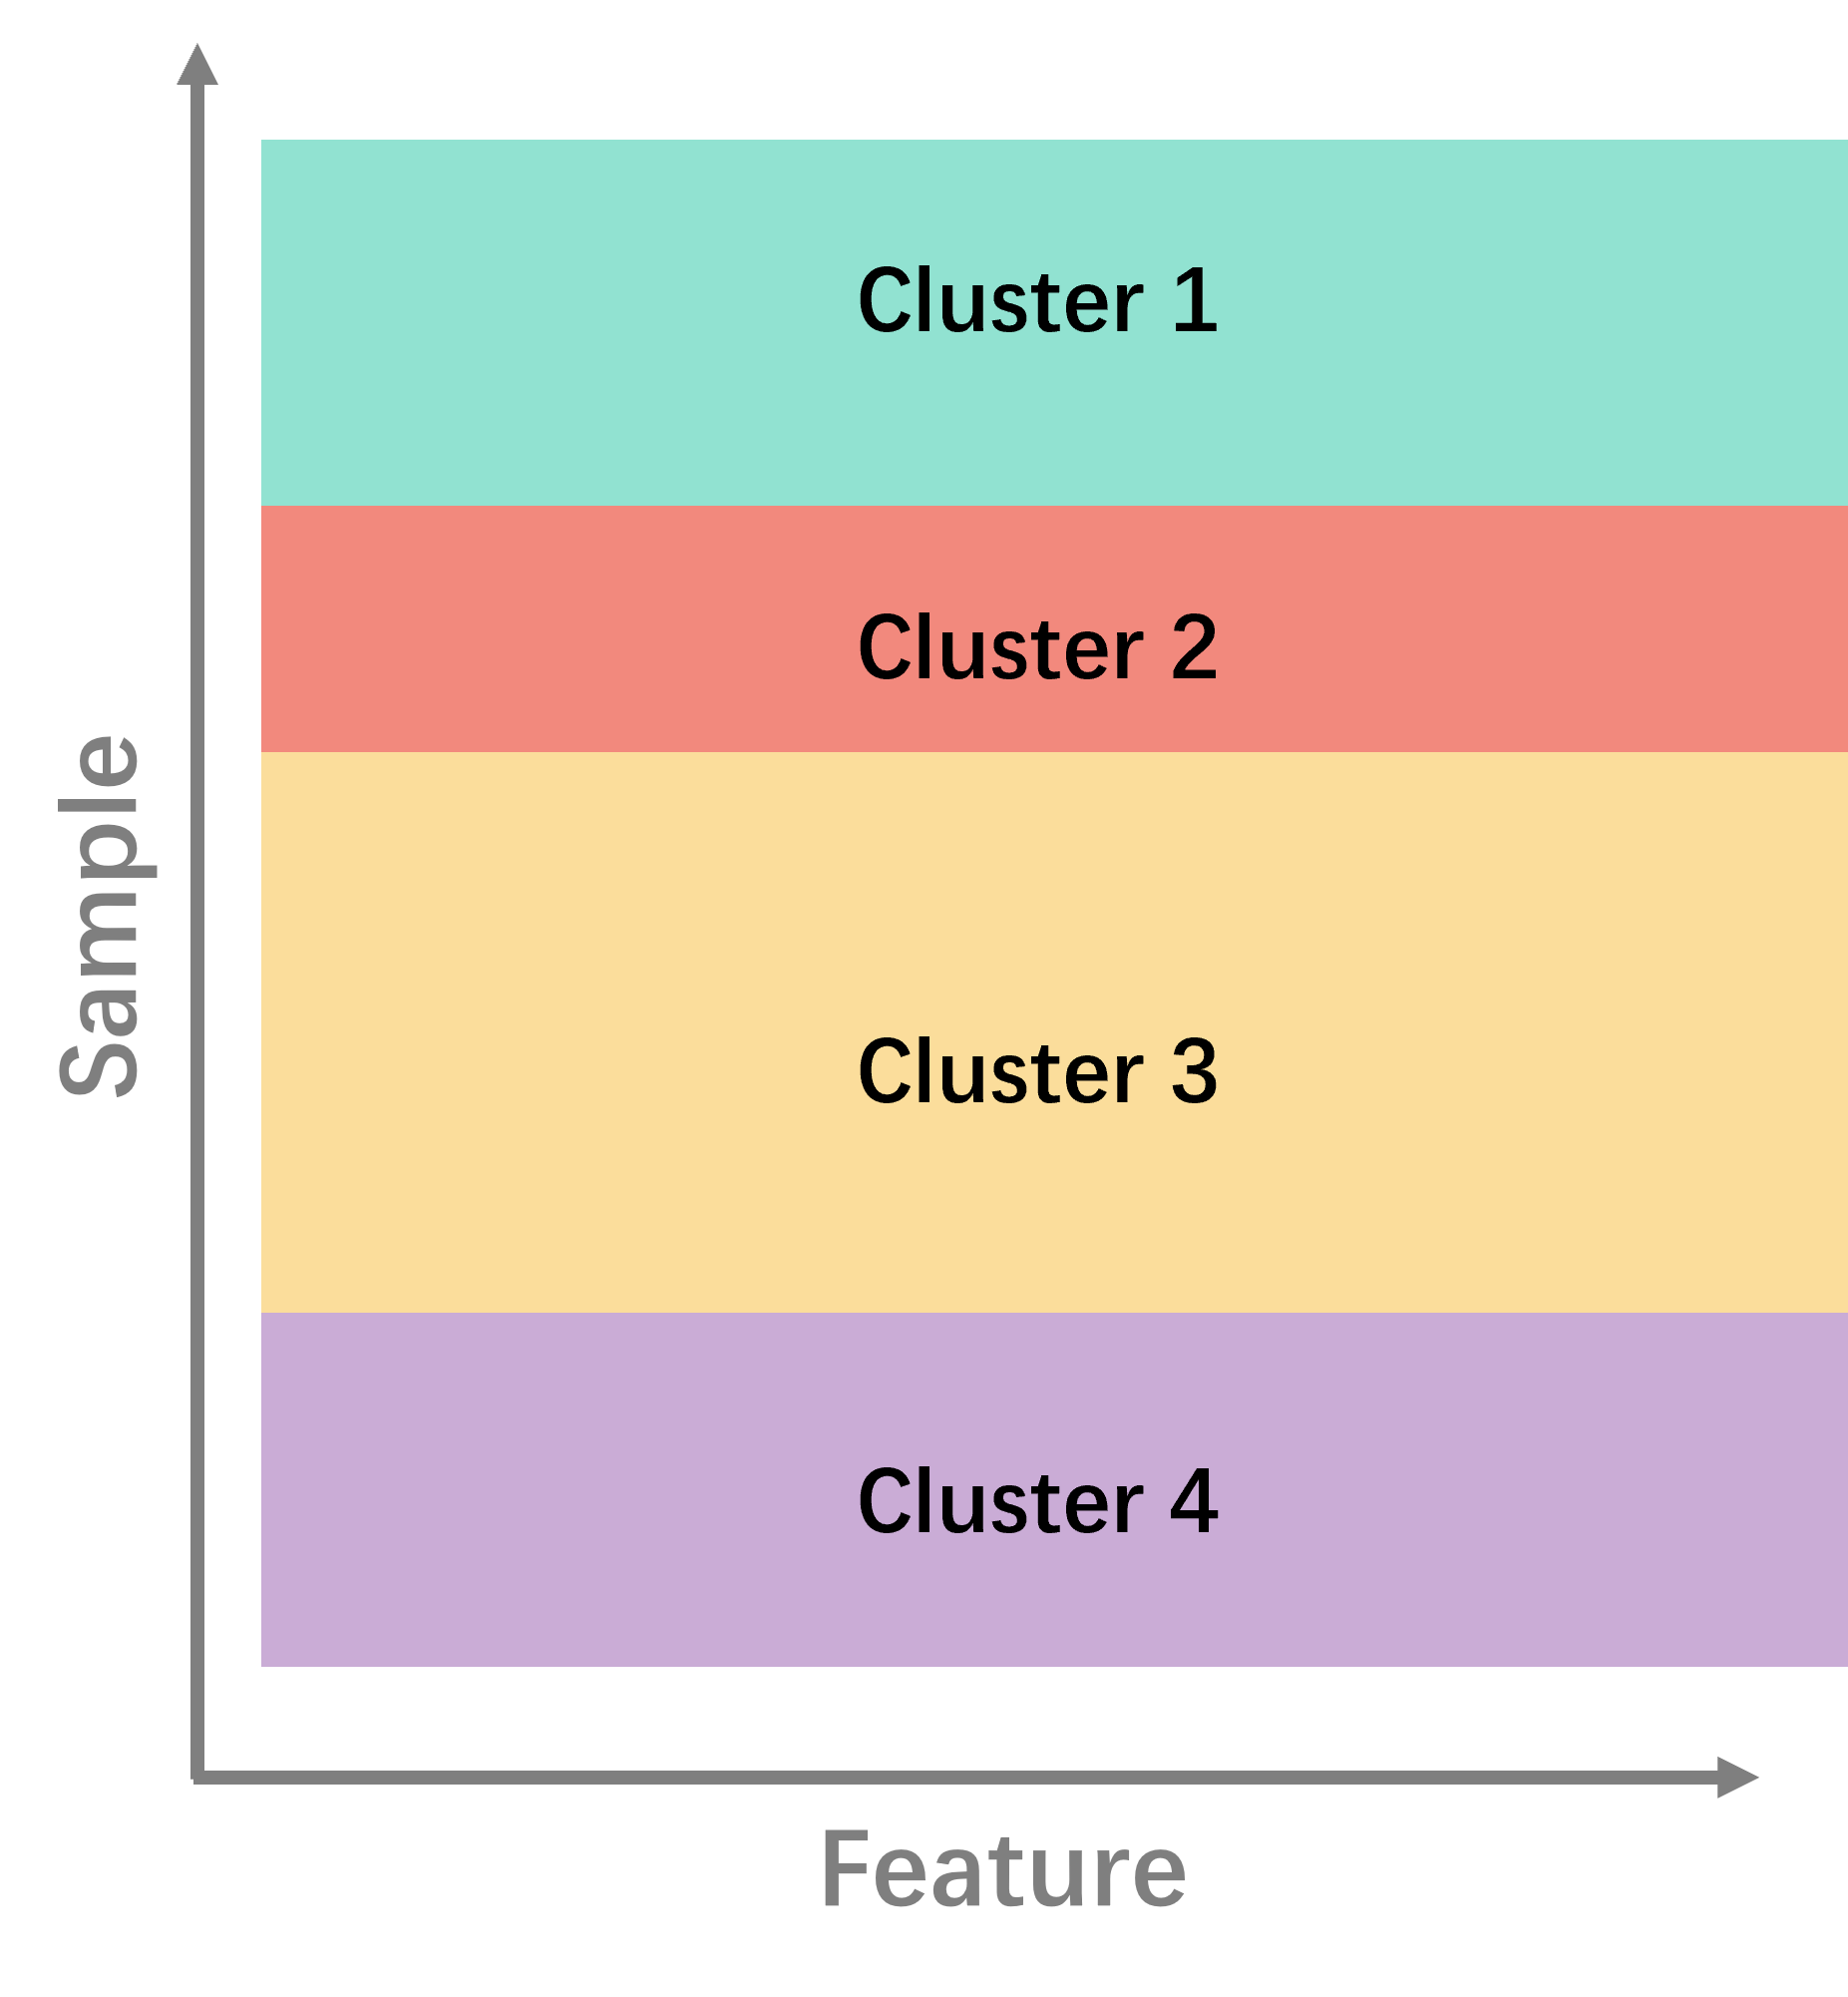
\includegraphics[width=\linewidth]{cluster.png}
        \caption{Clustering}
        \label{fig:cluster}
    \end{subfigure}
    \hfill
    \begin{subfigure}[b]{0.22\textwidth}
        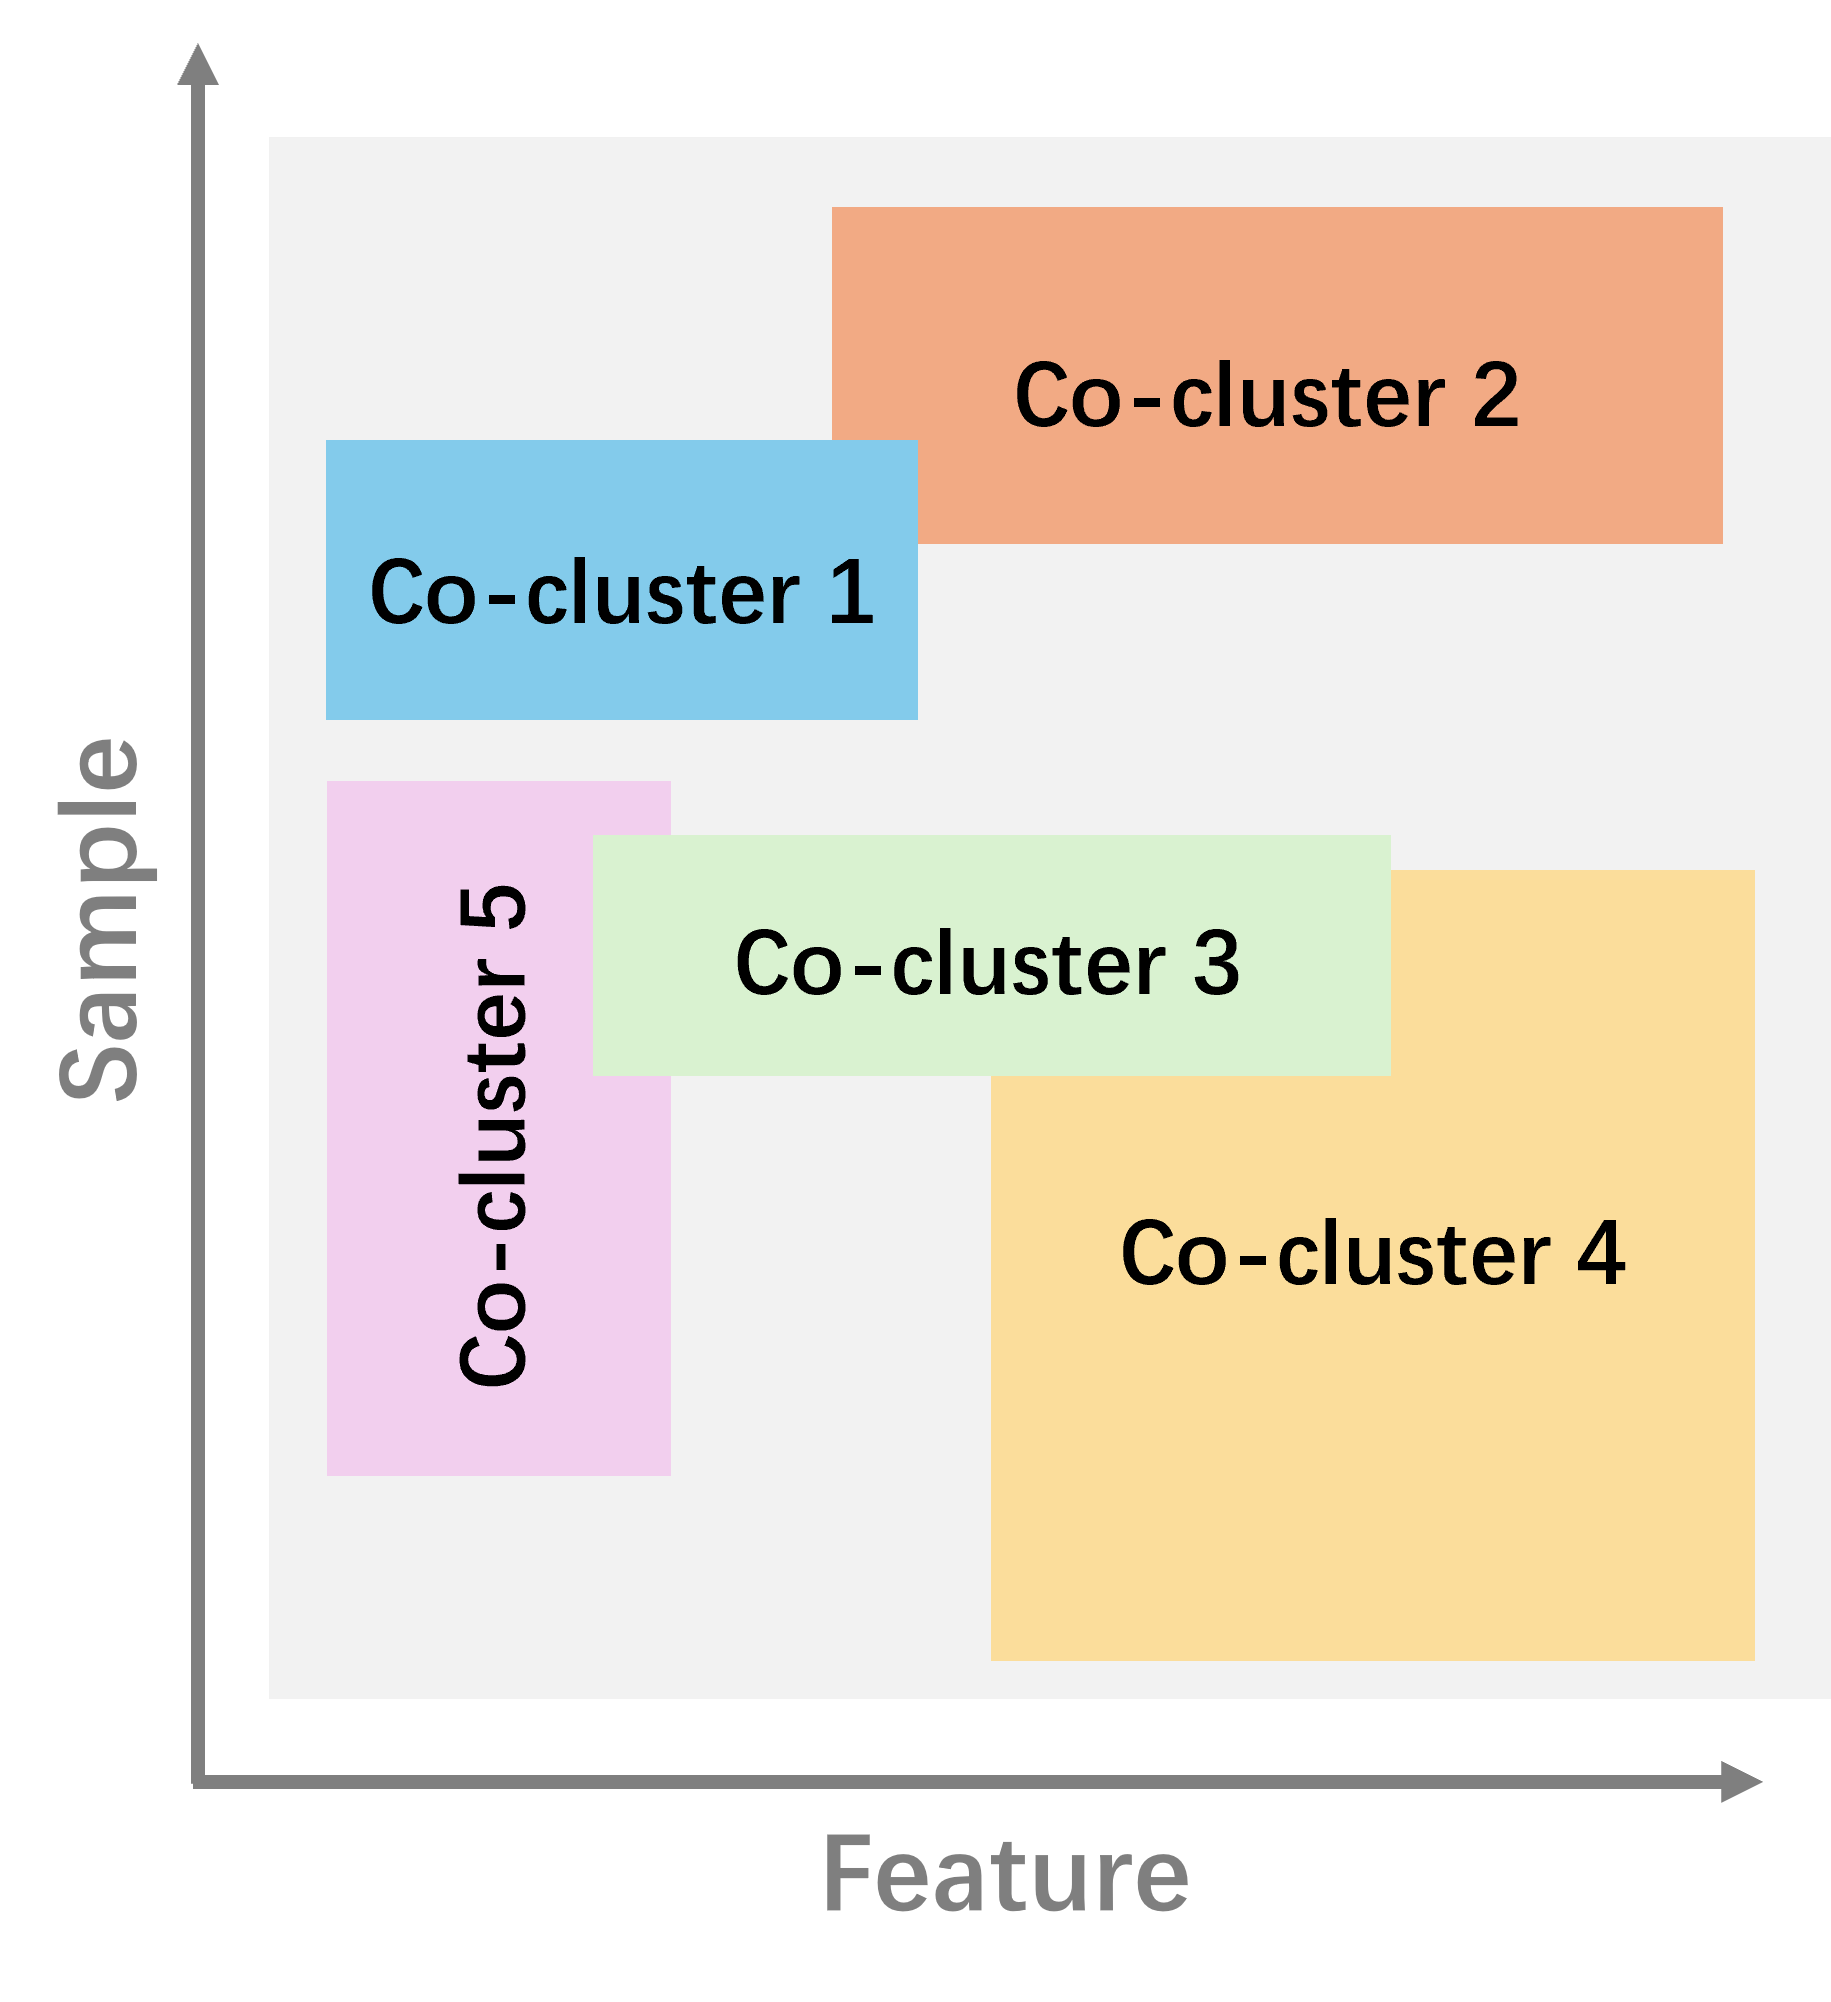
\includegraphics[width=\linewidth]{coc.png}
        \caption{Co-clustering}
        \label{fig:cocluster}
    \end{subfigure}
    \caption{An illustration of the differences between (a) Clustering and (b) Co-clustering~\cite{yan2017CoclusteringMultidimensionalBig}.}
    \label{fig:cocomparison}
\end{figure}

While co-clustering has great potential, existing co-clustering algorithms are impractical for handling large-scale data due to scalability and high complexity issues~\cite{cheng2015CoClusterDDistributedFramework}. This complexity arises from the need to simultaneously optimize both row and column clusters, turning the problem into a multi-objective optimization task. This task involves minimizing multiple loss functions concurrently, often resulting in conflicting gradients and optimization paths. These conflicts complicate the convergence process, making it difficult to achieve efficient and effective clustering~\cite{coello2007EvolutionaryAlgorithmsSolving}.
Our method, \emph{DiMergeCo}, takes inspiration from distributed map-reduce paradigms. Just as cartographers divide continents into manageable tiles without splitting mountain ranges, our probabilistic partitioning preserves co-cluster integrity. Local teams (parallel nodes) then chart each tile, while a hierarchical merging process (akin to stitching satellite imagery) reconstructs the global landscape—all without requiring a central "master cartographer." Unlike PNMTF~\cite{chen2023ParallelNonNegativeMatrix}, which requires broadcasting large matrices, our method uses probabilistic guarantees to minimize communication. Compared to Co-ClusterD~\cite{cheng2015CoClusterDDistributedFramework}, \emph{DiMergeCo} eliminates main-thread bottlenecks by distributing tasks across multiple nodes. To address these scalability limitations, PNMTF~\cite{chen2023ParallelNonNegativeMatrix} employs parallelization using distributed computing frameworks. However, it lacks guaranteed iteration numbers and requires broadcasting a non-adaptive scale matrix, which limits its scalability. Similarly, Co-ClusterD~\cite{cheng2015CoClusterDDistributedFramework}'s main thread must handle co-cluster statistics \(S_{cc}\), constraining its scalability. Despite attempts to distribute tasks, both algorithms still rely on the main thread to manage high-complexity tasks.

\textit{Co-clustering} overcomes traditional clustering's single-dimensional constraints through joint row-column grouping. While this paradigm shift enables multidimensional pattern discovery, existing co-clustering algorithms fail to scale for modern applications like genomics (millions of genes × thousands of conditions) and e-commerce (billions of user-item interactions). Current methods collapse due to: (1) Quadratic complexity in simultaneous optimization; (2) Centralized architectures that bottleneck distributed processing.

To address these gaps, we propose a two-stage framework that (1) dynamically partitions the matrix to preserve co-clusters and (2) hierarchically merges local results without central bottlenecks.

Our method is also modular, allowing seamless integration with existing co-clustering techniques. We implement our framework using MPI (Message Passing Interface) to distribute computational load across multiple nodes, significantly reducing processing time and computational demands. Our method is probabilistically guaranteed to converge, ensuring robustness and reliability across diverse datasets.

The proposed co-clustering method begins with our dynamic partitioning algorithm that divides the original data matrix into smaller submatrices. This partitioning facilitates parallel processing of co-clustering tasks across submatrices, significantly reducing both processing time and computational and storage demands for each processing unit. Our designed probabilistic model can determine the optimal number and configuration of these submatrices, ensuring comprehensive data coverage. If the atom co-clustering method is effective, this model guarantees that the entire framework will converge with an iteration number specified only by the scale of the data matrix, providing confidence in the robustness and reliability of our approach across diverse datasets.

Then, our hierarchical co-cluster merging algorithm iteratively combines the co-clusters from these submatrices. This process enhances the accuracy and reliability of the final co-clustering results and ensures robust and consistent clustering performance, particularly addressing issues of heterogeneity and model uncertainty. By leveraging a hierarchical merging strategy, we can efficiently integrate co-clusters without overwhelming any single processing unit, thereby maintaining scalability. Our method is modular, allowing any co-clustering method, including those with existing parallel designs, to be integrated seamlessly. This flexibility ensures that our approach can adapt and evolve with advancements in co-clustering techniques.

Our proposed method also includes a Message Passing Interface (MPI) implementation, which allows for effective distribution of the computational load across multiple nodes. The main computation node only needs to compute thresholds based on the size of the matrix, without requiring specialized performance beyond that of other nodes, making our approach more useful and scalable for large-scale applications. Unlike existing methods that require a high-performance central processing unit, our approach does not demand a supercomputer for the main thread. Additionally, our framework is probabilistically guaranteed to work.

The main contributions of this paper are as follows:
\begin{enumerate}
    \item \textbf{Dynamic Partitioning Algorithm:}
          Probabilistic model ensuring co-cluster integrity during distribution, breaking quadratic complexity

    \item \textbf{Hierarchical Merging Algorithm:}
          Communication-efficient aggregation avoiding central bottlenecks
    \item \textbf{MPI Implementation and Performance Evaluation:}
          Empirically validated framework showing linear scaling on billion-scale datasets"
\end{enumerate}

The remainder of this paper is organized as follows. Section \Cref{sec:related_work} discusses related work in the field of co-clustering and parallel computing. Section \Cref{sec:problem_formulation} presents the mathematical formulation and problem statement of co-clustering. Section \Cref{sec:proposed_model} details our proposed scalable co-clustering method.
Section \Cref{sec:experiment} presents the experimental evaluation of our method. Section \Cref{sec:conclusion} concludes the paper and outlines future research directions. The theoretical analysis, including error bounds, complexity analysis, and optimality conditions, is provided in \Cref{sec:appendix_theoretical_analysis} in the appendix.

\section{Related Work}
\label{sec:related_work}
\subsection{Co-clustering Models}

The concept of \emph{biclustering}, a special case of co-clustering for two-dimensional (2D) data, where both the rows and columns of data are clustered simultaneously, was first introduced by Hartigan~\cite{hartigan1972DirectClusteringData} to analyze gene expression data. This pioneering approach recognized the importance of simultaneously considering multiple dimensions of data to uncover more nuanced patterns.

Spectral Co-clustering with Singular Value Decomposition (SVD), introduced by Dhillon \textit{et al.}~\cite{dhillon2001CoclusteringDocumentsWords}, became widely adopted due to its straightforward implementation and effectiveness. This method leverages the mathematical properties of SVD to identify clusters by analyzing the principal components of the data matrix. Spectral co-clustering has since become a foundational technique, inspiring two main branches in co-clustering research: graph-based and matrix factorization-based approaches.

The most widely used graph-based co-clustering method is the Flexible Bipartite Graph Co-clustering (FBGPC)~\cite{chen2023FastFlexibleBipartitea}. FBGPC applies a flexible bipartite graph model directly to the original data, allowing for the simultaneous clustering of two distinct sets of objects, such as users and items in a recommendation system. This approach effectively captures the interactions between these sets, providing deeper insights into their relationships.

In contrast, Non-negative Matrix Tri-Factorization (NMTF)~\cite{long2005CoclusteringBlockValue} represents a leading matrix factorization-based method. NMTF decomposes the data matrix into multiple non-negative matrices, which correspond to the underlying factors of the data. By independently clustering both samples and features, NMTF reveals the latent structures within the data. This method has proven to be particularly useful in applications where the interpretability of factors is crucial, such as bioinformatics and social network analysis. Our method is orthogonal to NMTF, allowing for potential integration to enhance co-clustering efficiency.

Another innovative method, Deep Co-Clustering (DeepCC)~\cite{dongkuanxu2019DeepCoClustering}, combines the power of deep learning with traditional clustering techniques. DeepCC integrates deep autoencoders with Gaussian Mixture Models to improve the clustering of complex data. The autoencoders reduce the dimensionality of the data while preserving essential features, and the Gaussian Mixture Models identify clusters within this reduced space. Despite its advancements, DeepCC struggles with computational efficiency, particularly with diverse data types and iterative processes dependent on data sparsity. The deep learning components introduce additional layers of computation, which can be resource-intensive and time-consuming.

\subsection{Parallelizing Co-clustering}

To address the significant computational challenges posed by big data, parallel co-clustering methods have emerged as a vital solution. Parallelization leverages distributed computing frameworks to divide the computational load across multiple processors or machines, thereby improving scalability and efficiency.

Cheng \textit{et al.}~\cite{cheng2015CoClusterDDistributedFramework} introduced a distributed co-clustering framework, Co-ClusterD, which utilizes an Alternating Minimization Co-clustering (AMCC) algorithm with sequential updates. Co-ClusterD partitions the data into smaller chunks, which are processed in parallel, and then combines the results. However, this method faces challenges with guaranteed convergence. The iterative nature of AMCC, coupled with the need for sequential updates, can lead to inefficiencies and bottlenecks, particularly as the size and complexity of the data increase.

While matrix factorization techniques have shown promise for co-clustering large datasets, scaling these algorithms for massive high-dimensional data remains an open challenge. Chen \textit{et al.}~\cite{chen2023ParallelNonNegativeMatrix} proposed a parallel non-negative matrix tri-factorization (PNMTF) method that distributes computation across multiple nodes to accelerate factorizations. PNMTF decomposes the original matrix into simpler, non-negative components, which are then processed in parallel. However, even these advanced methods encounter difficulties with extremely large datasets. The need to broadcast intermediate results and synchronize updates across nodes introduces significant communication overhead, which can negate the benefits of parallelization.

Existing co-clustering algorithms~\cite{chen2023ParallelNonNegativeMatrix, cheng2015CoClusterDDistributedFramework} rely on a central processing thread to handle complex tasks like managing co-cluster statistics. This centralization creates a bottleneck, significantly limiting their scalability and making them impractical for large-scale datasets. Additionally, the dual-focus analysis of co-clustering, which simultaneously optimizes row and column clusters, requires evaluating a vast number of potential relationships. This complexity can grow exponentially with the size of the data, making it impractical for large-scale applications.

In contrast, our proposed method adopts a divide-and-conquer strategy to overcome these limitations. By partitioning the input matrix into smaller submatrices, we reduce the dimensionality of each individual task, making them more manageable. Each submatrix is co-clustered in parallel, leveraging distributed computing resources to expedite the process. This technique reduces the complexity imposed by high dimensionality and minimizes the communication overhead associated with broadcasting and synchronization. The separate co-clustering results from each submatrix are then combined using a hierarchical merging algorithm to form the final co-clusters. This novel approach addresses the computational challenges inherent in co-clustering large-scale data and introduces a scalable solution tailored for big data.

\section{Problem Formulation}
\label{sec:problem_formulation}

\subsection{Notations and Definitions}
Let $\mathbf{A} \in \mathbb{R}^{m \times n}$ be a data matrix, where $m$ and $n$ denote the number of samples and features, respectively. We assume that there are $k$ row clusters and $d$ column clusters to be identified simultaneously, resulting in $k \times d$ co-clusters. Each element $a_{ij}$ represents the interaction (or similarity) between the $i$-th sample and the $j$-th feature.

We define:
\begin{itemize}
    \item $I = \{1,2,\ldots,m\}$ and $J = \{1,2,\ldots,n\}$ as the sets of row and column indices.
    \item $\mathcal{C} = \{\mathbf{C}_1, \mathbf{C}_2, \ldots, \mathbf{C}_K\}$ as the set of discovered co-clusters, where each $\mathbf{C}_k \subseteq I \times J$ is a submatrix that exhibits coherent patterns.
    \item $\mathbf{Y} \in \mathbb{R}^{n \times c}$ as the indicator matrix, where each row contains exactly one element equal to 1 and all other elements equal to 0.
    \item $\|\mathbf{A}\|_F = \sqrt{\sum_{i=1}^m \sum_{j=1}^n a_{ij}^2}$ as the Frobenius norm of matrix $\mathbf{A}$.
\end{itemize}

\subsection{Mathematical Formulation of Co-clustering}
Co-clustering is a method designed to simultaneously group a set of rows and columns in a data matrix $\mathbf{A} \in \mathbb{R}^{M \times N}$, where $M$ denotes the number of features or variables and $N$ denotes the number of samples or objects. Each element $a_{ij}$ in the matrix at the $(i, j)$-th position represents the relationship or measurement between the $i$-th sample and the $j$-th feature. The primary goal of co-clustering is to identify subsets of rows ($I\subseteq \{1, 2, \ldots, M\}$) and columns ($J\subseteq \{1, 2, \ldots, N\}$) into homogenous submatrices, $\mathbf{A}_{I, J}$, that exhibit distinctive patterns or uniform characteristics, thus forming coherent co-clusters~\cite{zhao2017DetectionCorrelatedCoclusters}. The objective is to partition $\mathbf{A}$ into $k$ row clusters and $d$ column clusters, resulting in $k \times d$ distinct co-clusters. Note that if we find all low-rank submatrices, and after evaluating its Pearson correlation coefficient, we can find the co-clusters~\cite{zhao2016IdentifyingMultidimensionalCoclusters}. When rows and columns are optimally reordered, $\mathbf{A}$ can be visualized as a blocked-matrix, where each block represents a co-cluster with higher similarity within than between blocks as show in \Cref{fig:cocluster}.

To evaluate if a submatrix $\mathbf{A}_{I, J}$ forms a coherent co-cluster, we define a score function \( f(\mathbf{A}_{I, J}) \) that quantifies the homogeneity of the submatrix.

\begin{definition}[Singular Value Ratio Score]
    \label{def:co_cluster}
    Consider a matrix \(\mathbf{A} \in \mathbb{R}^{M \times N}\). The Singular Value Ratio Score is defined as follows:
    \begin{itemize}
        \item For a given submatrix \(\mathbf{A}\), the Singular Value Ratio Score is given by:
              \begin{equation}
                  s(\mathbf{A}) = \frac{s_1}{s_2},
              \end{equation}
              where \(s_1\) is the largest singular value of \(\mathbf{A}\) and \(s_2\) is the second largest singular value of \(\mathbf{A}\).
        \item For a given submatrix \(\mathbf{A}\), the normalized Singular Value Ratio Score is defined as:
              \begin{equation}
                  S(\mathbf{A}) = \frac{s(\mathbf{A})}{\|\mathbf{A}\|_F},
              \end{equation}
              where \(\|\mathbf{A}\|_F\) denotes the Frobenius norm of \(\mathbf{A}\).
    \end{itemize}
\end{definition}

\subsection{Original Co-Clustering Problem}
Co-clustering can be formulated as a constrained optimization problem. Given a normalized similarity matrix $\mathbf{S}$ derived from $\mathbf{A}$, we seek to minimize:
\begin{equation}
    \label{eq:objective}
    \min_{\mathbf{F}^T \mathbf{F} = \mathbf{I}} J(\mathbf{F}) = -\text{Tr}\left(\mathbf{F}^T \mathbf{D}_{\mathbf{A}}^{-1/2}\mathbf{A}\mathbf{D}_{\mathbf{A}}^{-1/2}\mathbf{F}\right)
\end{equation}
where:
\begin{itemize}
    \item $\mathbf{D}_{\mathbf{A}}$ is a degree-like diagonal matrix
    \item $\mathbf{F}$ is the cluster indicator matrix subject to orthogonality constraints
    \item $\text{Tr}(\cdot)$ denotes the matrix trace operator
\end{itemize}

The objective seeks a partitioning that maximizes coherence within co-clusters while minimizing inter-cluster overlaps. This can be equivalently expressed as a graph partitioning problem:
\begin{equation}
    \min_{\mathbf{Y} \in \text{Ind}} \sum_{l=1}^c \frac{\mathbf{y}_l^T \mathbf{L}_\mathbf{A}\mathbf{y}_l}{\mathbf{y}_l^T \mathbf{D}_\mathbf{A} \mathbf{y}_l},
\end{equation}
where $\mathbf{L}_\mathbf{A} = \mathbf{D}_\mathbf{A} - \mathbf{A}$ is the graph Laplacian matrix.

\subsection{Challenges in Large-Scale Settings}
For very large $m$ and $n$, several critical challenges emerge. The optimization problem involves matrix operations with complexity $O(mn\min(m,n))$, making direct computation prohibitively expensive for large matrices. Storage and manipulation of the full similarity matrix requires $O(mn)$ memory, which often exceeds available resources for large-scale problems. Additionally, intermediate factors during optimization may require significant additional memory. In distributed or parallel settings, broadcasting large matrices and synchronizing updates across nodes incurs substantial communication costs, scaling quadratically with matrix dimensions. The non-convex nature of the optimization problem becomes more pronounced with increasing dimensionality, making it harder to find stable solutions.

\section{The Scalable Co-clustering Method}
\label{sec:proposed_model}

In this section, we propose a scalable co-clustering method, called \emph{Divide-and-Merge Co-Clustering } (DiMergeCo), which is designed to handle large datasets by dividing the original matrix into smaller submatrices and subsequently merging local co-clustering results. The approach addresses the two core challenges of large-scale data analysis: scalability and accuracy. \Cref{fig:DiMergeCo_pipeline} shows a conceptual illustration of the framework, where each large dataset is split into multiple blocks for efficient parallel co-clustering. Once local results are obtained, a hierarchical merging step refines and unifies these partial solutions into a globally consistent set of co-clusters.

\begin{figure*}[t]
    \centering
    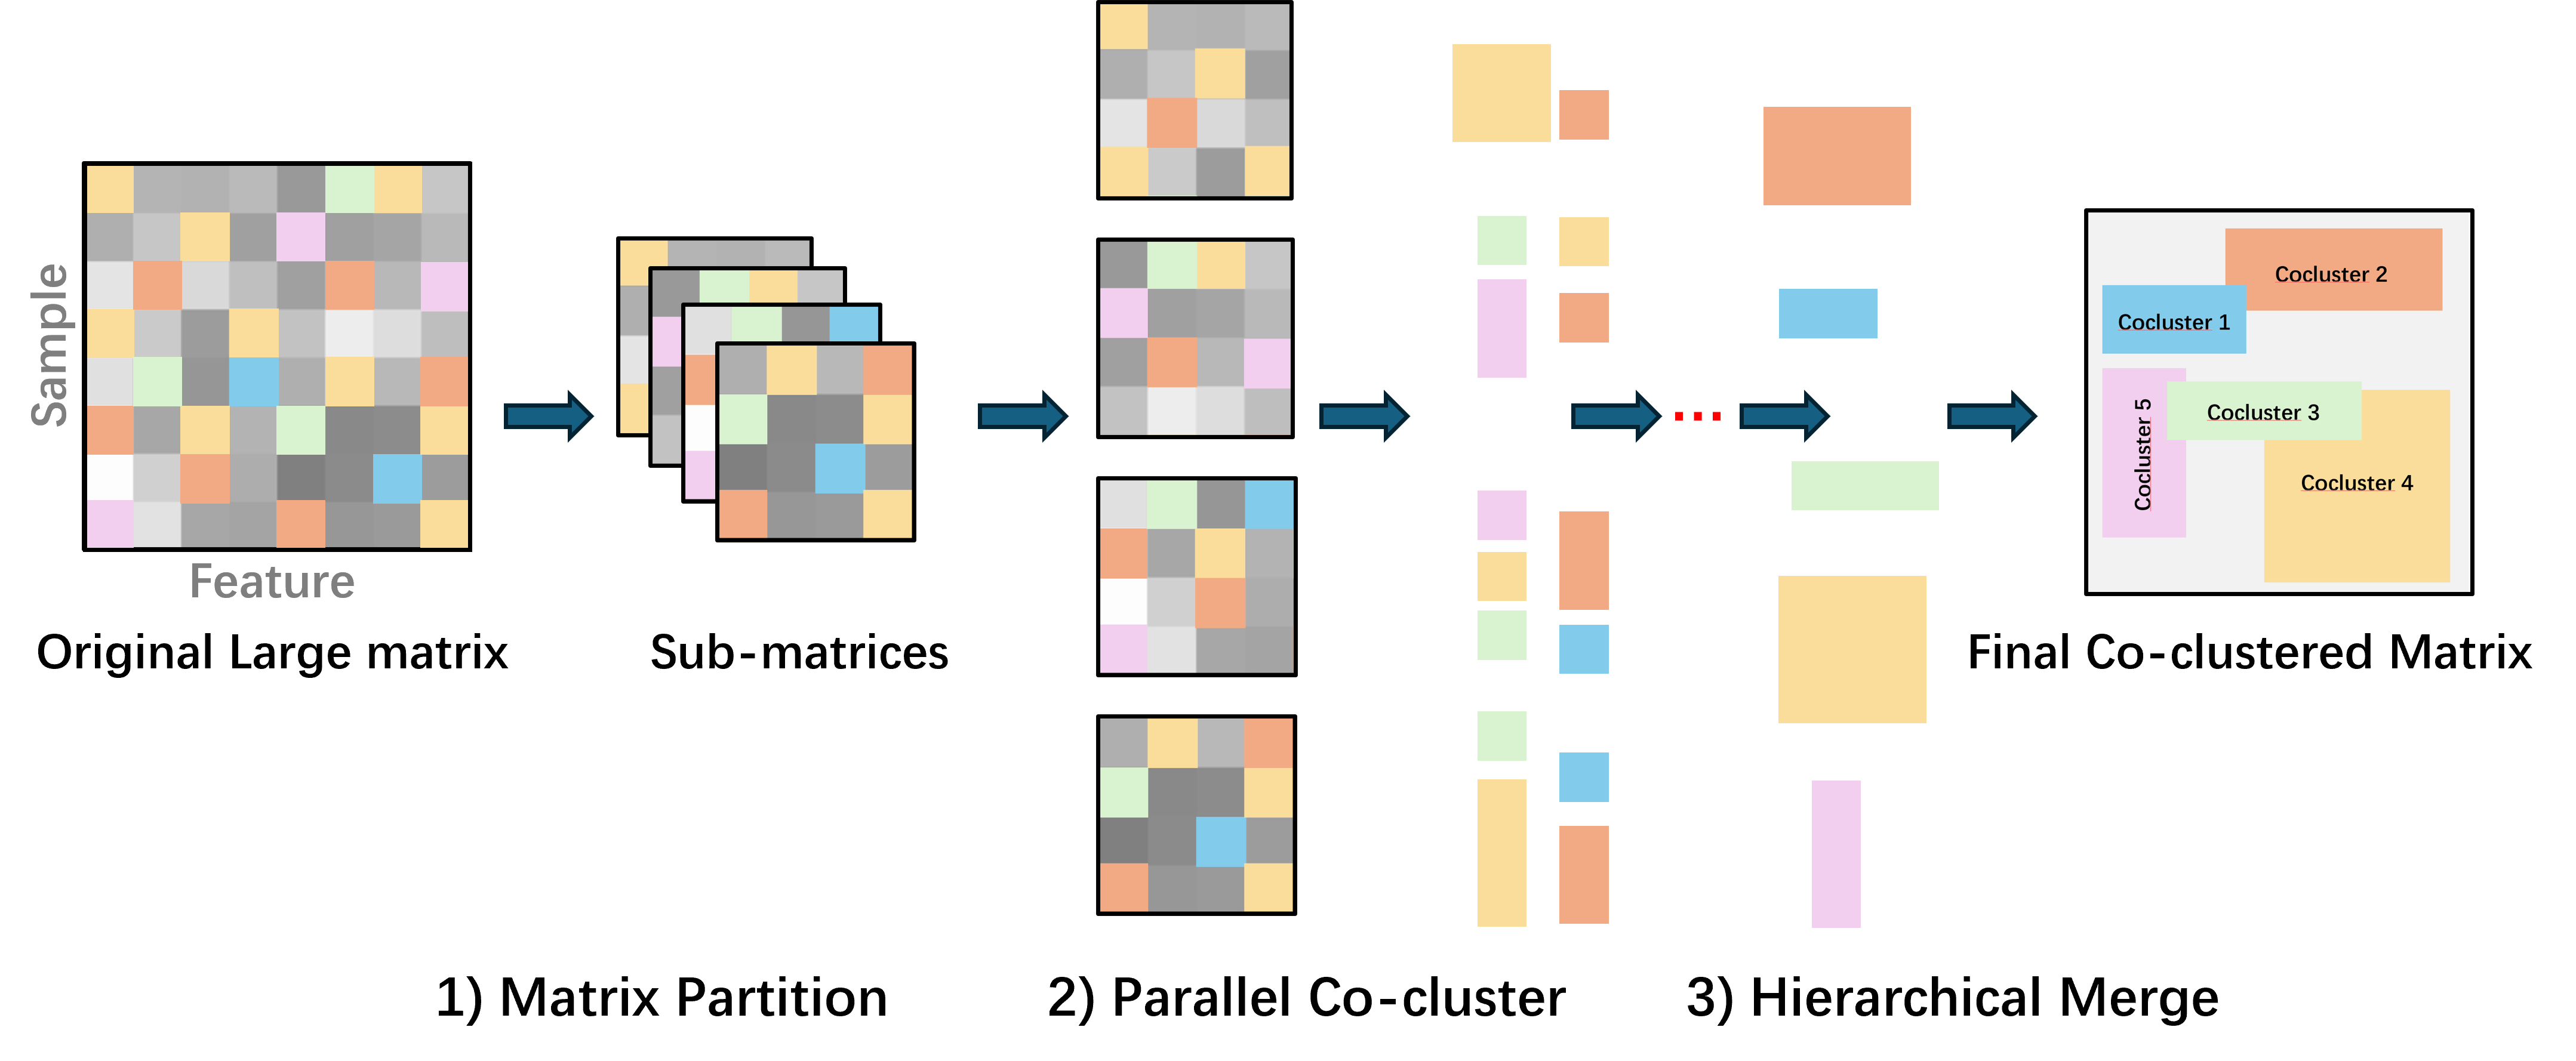
\includegraphics[width=0.8\linewidth]{workflow.png} % replace with your figure file
    \caption{High-level pipeline of the DiMergeCo framework. The data matrix is first partitioned into smaller blocks, each block is locally co-clustered in parallel, and the partial results are merged hierarchically to form the final co-clusters.}
    \label{fig:DiMergeCo_pipeline}
\end{figure*}

\subsection{Motivation}
\label{subsec:motivation}

Our approach is grounded in a fundamental property of matrix algebra: any submatrix necessarily inherits a rank no greater than its parent matrix~\cite{horn1985MatrixAnalysis}. Formally, this can be stated as:

\begin{theorem}[Rank Monotonicity of Submatrices]
    \label{thm:rank_monotonicity}
    For any matrix $A \in \mathbb{R}^{m \times n}$ and its submatrix $A'$, we have $\text{rank}(A') \leq \text{rank}(A)$.
\end{theorem}

This property provides a theoretical guarantee that when we partition a matrix containing low-rank structures, these patterns remain discoverable within the resulting submatrices. Building on this foundation, co-clustering aims to identify groups of rows and columns that form relatively low-rank submatrices in a data matrix. Such submatrices, which we refer to as co-clusters, often represent the core relationships or patterns within high-dimensional datasets. In practice, however, large and intricate data can obscure these low-rank structures, making them challenging to detect through a single global procedure. Dividing the dataset into smaller submatrices can be highly beneficial for revealing localized low-rank patterns, since each submatrix—being smaller—tends to have an even lower rank (or be easier to approximate by low-rank factors). Many existing techniques, such as singular value decomposition or non-negative matrix factorizations, work more efficiently and accurately on these smaller blocks.

Although splitting the matrix might initially risk cutting through a co-cluster, our framework mitigates this concern by probabilistically ensuring that any sufficiently large or dense co-cluster remains intact in at least one block with high probability. This probabilistic assurance aligns with recent advances in dynamic partitioning strategies for distributed systems~\cite{huang2024EnergyAwareIntegratedNeural}, where adaptive resource allocation has proven critical for maintaining structural integrity under resource constraints. After local low-rank submatrices are discovered, a hierarchical merging procedure effectively reassembles partial co-clusters into cohesive global structures. This combination step reclaims the larger low-rank patterns and produces final co-clusters that capture coherent relationships across the original dataset. By coordinating local discovery of smaller low-rank blocks and merging them to form full co-clusters, the proposed approach both preserves essential structure and scales to large data.

Unlike Co-ClusterD~\cite{cheng2015CoClusterDDistributedFramework}, which statically partitions matrices risking co-cluster fragmentation,.\emph{DiMergeCo}'s adaptive resizing (Lines 7--9, \Cref{alg:partitioning}) dynamically adjusts block dimensions to preserve co-clusters with probabilistic guarantees (\Cref{thm:probability_co_cluster_detection}).

\subsection{Overview}
\label{subsec:overview}
Our method involves partitioning large matrices into smaller, manageable submatrices guided by a probabilistic model. This ensures that co-cluster integrity is maintained during division, addressing the risk of missing small or intricate co-clusters by estimating the likelihood of their identification. Consequently, the model guarantees comprehensive data coverage and robust clustering results.

Each submatrix then undergoes independent co-clustering analysis. Our framework is modular, allowing the integration of any advanced co-clustering technique that can reliably identify co-clusters above a certain size. This flexibility ensures that the method can be tailored to the unique characteristics of each submatrix, optimizing clustering results.

Additionally, a crucial theorem underpins our approach by guaranteeing the success probability of the framework. As long as the chosen co-clustering method effectively identifies all co-clusters above the specified size with high probability, our overall method maintains its theoretical guarantees of comprehensive and accurate clustering outcomes.

Finally, a novel hierarchical merging strategy combines the co-clustering results from all submatrices into a coherent global solution. This integration provides fine-grained insights into each submatrix and enhances the overall accuracy and reliability of the co-clustering results.

The hierarchical merging process iteratively combines co-clusters from the submatrices, ensuring that the final result is both comprehensive and consistent across the entire dataset. Unlike existing methods such as Non-negative Matrix Tri-Factorization (NMTF) or alternating row and column optimization approaches~\cite{wang2011FastNonnegativeMatrix}, our merging process has a bounded iteration count determined by the data size. This bounding leads to a predictable time frame for achieving the ideal result, ensuring computational efficiency.

This multi-step approach not only improves scalability but also guarantees that the final co-clustering results are robust and reliable, even for very large datasets. The complete procedure is detailed in \Cref{alg:method}.

\begin{algorithm}[!t]
    \caption{Optimal Matrix Partition and Hierarchical Co-cluster Merging Method}\label{alg:method}
    \begin{algorithmic}[1]
        \REQUIRE{Data matrix $\mathbf{A} \in \mathbb{R}^{M \times N}$, Co-cluster set $C = \{C_k\}_{k=1}^K$, Block sizes $\{\phi_i\}_{i=1}^m$, $\{\psi_j\}_{j=1}^n$, Thresholds $T_m$, $T_n$, Sampling times $T_p$, Probability threshold $P_\text{thresh}$;}
        \ENSURE{Co-clustered result $\mathcal{C}$;}
        \STATE Initialize block set $B = \{B_{(i,j)}\}_{i=1}^m,_{j=1}^n$ based on $\phi_i$ and $\psi_j$
        \STATE Calculate $s^{(k)}$ and $t^{(k)}$ for each co-cluster $C_k$
        \FOR{$k=1$ to $K$}
        \STATE Calculate $P(\omega_k)$ for co-cluster $C_k$
        \IF{$P(\omega_k) < P_\text{thresh}$}
        \STATE Partition matrix $A$ into blocks $B$ and perform co-clustering
        \STATE Aggregate co-clustered results from each block
        \ENDIF
        \ENDFOR
        \RETURN Aggregated co-clustered result $\mathcal{C}$
    \end{algorithmic}
\end{algorithm}

In \Cref{sec:proposed_model}, we detail the three core components of DiMergeCo: the large matrix partitioning algorithm (\Cref{subsec:large_matrix_partitioning}), the local co-clustering method (\Cref{subsec:local_co_clustering}), and the hierarchical merging strategy (\Cref{subsec:hierarchical_merging}). Each component is designed to address specific challenges in large-scale co-clustering while maintaining theoretical guarantees. For completeness, we also present a graph-based spectral co-clustering variant that can be seamlessly integrated into our framework. The theoretical foundations supporting these components are then presented in \Cref{sec:theoretical_foundations}, including convergence analysis and error bounds. Finally, we demonstrate the practical effectiveness of our approach through an MPI implementation for distributed computing environments in \Cref{subsec:mpi_implementation}.

\subsection{Large Matrix Partitioning}
\label{subsec:large_matrix_partitioning}
The primary challenge in co-clustering large matrices is the risk of losing meaningful co-cluster relationships when the matrix is partitioned into smaller submatrices. To address this, we introduce an optimal partitioning algorithm underpinned by a probabilistic model. This model is meticulously designed to navigate the complexities of partitioning, ensuring that the integrity of co-clusters is maintained even as the matrix is divided. The objective of this algorithm is twofold: to determine the optimal partitioning strategy that minimizes the risk of fragmenting significant co-clusters and to define the appropriate number of repartitioning iterations needed to achieve a desired success rate of co-cluster identification.

\subsubsection{Partitioning and Repartitioning Strategy based on the Probabilistic Model}

Our probabilistic model serves as the cornerstone of the partitioning algorithm. It assures all co-clusters above a demarcated size threshold are identified with a high probability, guiding the partitioning process to minimize the risk of losing critical co-cluster relationships. The model is based on the following assumptions:

In the scenario where the matrix $A$ is partitioned into $m \times n$ blocks, each block has size $\phi_i \times \psi_j$, that is, $M=\sum_{i=1}^m \phi_i$ and $N=\sum_{j=1}^n \psi_j$, the joint probability of $M_{(i,j)}^{(k)}$ and $N_{(i,j)}^{(k)}$ is given by \Cref{thm:joint_probability}:
\begin{equation}
    \begin{split}
        P(M_{(i,j)}^{(k)} & < T_m, N_{(i,j)}^{(k)} < T_n)                                                                           \\
                          & = \sum_{\alpha=1}^{T_m-1} \sum_{\beta=1}^{T_n-1} P(M_{(i,j)}^{(k)} = \alpha) P(N_{(i,j)}^{(k)} = \beta) \\
                          & \le \exp[-2 (s_i^{(k)})^2 \phi_i + -2 (t_j^{(k)})^2 \psi_j\rbrack
    \end{split}
\end{equation}
where $s_i^{(k)}$ and $t_j^{(k)}$ are the minimum row and column sizes of co-cluster $C_k$ in block $B_{(i,j)}$, the size of the co-cluster $C_k$ is $M^{(k)} \times N^{(k)}$, and $M^{(k)}$ and $N^{(k)}$ are the row and column sizes of co-cluster $C_k$, respectively.

Thus, $P$, the probability of identifying all co-clusters is given by \Cref{thm:probability_co_cluster_detection}:

\begin{equation}
    \begin{split}
        P \ge 1 - \exp \left\{ -2 T_p \lbrack \phi m (s^{(k)})^2 + \psi n (t^{(k)})^2\rbrack  \right\} \label{eq:prob_of_identifying_all_co_clusters}
    \end{split}
\end{equation}
where $P(\omega_k)$ is the probability of the failure of identifying co-cluster $C_k$, $T_p$ is the number of sampling times, $\phi$ and $\psi$ are the row and column block sizes, and $s^{(k)}$ and $t^{(k)}$ are the minimum row and column sizes of co-cluster $C_k$.

\Cref{eq:prob_of_identifying_all_co_clusters} is central to our algorithm for partitioning large matrices for co-clustering, providing a probabilistic model that informs and optimizes our partitioning strategy to preserve co-cluster integrity. It mathematically quantifies the likelihood of identifying all relevant co-clusters within partitioned blocks, guiding us to mitigate risks associated with partitioning that might fragment vital co-cluster relationships.

Based on \Cref{eq:prob_of_identifying_all_co_clusters}, we can establish a constraint between the partitioning time $T_p$ and the partition solution $Par(\{\phi_i\}_{i=1}^m, \{\psi_j\}_{j=1}^n)$, ensuring that the partitioning strategy adheres to a predetermined tolerance success rate, thereby minimizing the risk of co-cluster fragmentation.

\subsubsection{Probabilistic Model for Partitioning}
\label{subsec:probabilistic_model}
\begin{lemma}[Joint Probability of Co-cluster Size]
    \label{thm:joint_probability}
    Let $C_k$ be a co-cluster and $B_{(i,j)}$ be a block in the partitioned matrix. The probability that the size of the co-cluster $C_k$ within block $B_{(i,j)}$ is less than $T_m$ rows and $T_n$ columns is given by:
    \begin{equation}
        P(M_{(i,j)}^{(k)} < T_m, N_{(i,j)}^{(k)} < T_n) \leq \exp\left[-2 (s_i^{(k)})^2 \phi_i -2 (t_j^{(k)})^2 \psi_j\right]
    \end{equation}
    where $s_i^{(k)} = \cfrac{M^{(k)}}{M} - \cfrac{T_m-1}{\phi_i}$ and $t_j^{(k)} = \cfrac{N^{(k)}}{N} - \cfrac{T_n-1}{\psi_j}$.
\end{lemma}

This lemma quantifies the likelihood that a co-cluster will remain sufficiently large within a given block, thereby preserving its detectability. By bounding the joint probability of both row and column dimensions of a co-cluster being below specified thresholds, we can systematically determine optimal block sizes that minimize the risk of fragmenting significant co-clusters.

\begin{theorem}[Probability of Co-cluster Detection]
    \label{thm:probability_co_cluster_detection}
    If the matrix $\mathbf{A}$ is partitioned into $m \times n$ blocks, each with sizes $\phi_i \times \psi_j$, and the probability of failing to detect co-cluster $\mathbf{C}_k$ in any block is $P(\omega_k)$, then
    \begin{equation}
        P \geq 1 - \exp \left\{ -2 T_p \left[ \phi m (s^{(k)})^2 + \psi n (t^{(k)})^2 \right] \right\}
    \end{equation}
    where $P(\omega_k)$ is the probability of failing to identify co-cluster $C_k$, $T_p$ is the number of sampling times, $\phi$ and $\psi$ are the row and column block sizes, and $s^{(k)}$ and $t^{(k)}$ are the minimum row and column sizes of co-cluster $C_k$.
\end{theorem}

Building on \Cref{thm:joint_probability}, this theorem provides a robust framework for estimating the probability of successfully detecting all significant co-clusters across multiple partitioning iterations. It enables us to set partitioning parameters that achieve a desired success rate, thereby ensuring that the co-clustering process remains both reliable and efficient.

These theoretical results directly inform our partitioning strategy by providing a mathematical foundation for selecting block sizes and determining the number of required partitioning iterations. As guaranteed by \Cref{thm:rank_monotonicity}, this partitioning strategy preserves the essential low-rank structures within the data, while the probabilistic bounds derived from \Cref{thm:probability_co_cluster_detection} ensure that co-clusters are detected with high probability.

\subsubsection{Practical Implementation of the Partitioning Strategy}
\label{subsec:practical_implementation}

The probabilistic model in \Cref{eq:prob_of_identifying_all_co_clusters} governs the trade-off between partitioning parameters and co-cluster detection reliability. To operationalize this, we formulate a constrained optimization problem:
\begin{equation}
    \begin{aligned}
         & \underset{\{\phi_i\}, \{\psi_j\}, T_p}{\text{Maximize}}
         &                                                         & P = 1 - \exp\left( -2 T_p \left[ \phi m (s^{(k)})^2 + \psi n (t^{(k)})^2 \right] \right)                                                                                                  \\
         & \text{subject to}
         &                                                         & T_p \leq T_{\text{max}}, \quad \sum_{i=1}^m \phi_i = M, \quad \sum_{j=1}^n \psi_j = N,                                                                                                    \\
         &                                                         &                                                                                          & \phi_i \geq \max(T_m, \epsilon M), \quad \psi_j \geq \max(T_n, \epsilon N), \quad \forall i,j,
    \end{aligned}
\end{equation}
where $\epsilon = 0.01$ prevents degenerate blocks, $\phi = \frac{1}{m}\sum \phi_i$ and $\psi = \frac{1}{n}\sum \psi_j$ are average block dimensions, and $s^{(k)} = \min_i \left( \frac{M^{(k)}}{M} - \frac{T_m-1}{\phi_i} \right)$, $t^{(k)} = \min_j \left( \frac{N^{(k)}}{N} - \frac{T_n-1}{\psi_j} \right)$ enforce detectability.

\begin{algorithm}[!t]
    \caption{Adaptive Matrix Partitioning for Co-Cluster Preservation}
    \label{alg:partitioning}
    \begin{algorithmic}[1]
        \REQUIRE{$M, N, T_m, T_n, T_{\text{max}}, P_{\text{thresh}}$}
        \ENSURE{$\{\phi_i\}, \{\psi_j\}, T_p$}
        \STATE Initialize $m \gets \lceil M / T_m \rceil$, $n \gets \lceil N / T_n \rceil$ \COMMENT{Minimum blocks to avoid fragmentation}
        \STATE $\phi_i \gets \lceil M/m \rceil$, $\psi_j \gets \lceil N/n \rceil$ $\forall i,j$ \COMMENT{Uniform initialization}
        \STATE Compute $s^{(k)}, t^{(k)}$ via \Cref{thm:joint_probability} for all $C_k$
        \STATE Calculate $P \gets 1 - \exp\left( -2 T_p \left[ \phi m (s^{(k)})^2 + \psi n (t^{(k)})^2 \right] \right)$
        \WHILE{$P < P_{\text{thresh}}$ \AND $T_p \leq T_{\text{max}}$}
        \FOR{each $C_k$ where $M^{(k)} \geq T_m$ \AND $N^{(k)} \geq T_n$}
        \STATE Identify blocks overlapping $C_k$ as $\mathcal{B}_k$
        \STATE $\phi_i \gets \max\left( \phi_i, \left\lceil \frac{M^{(k)} T_m}{M s^{(k)}} \right\rceil \right)$ $\forall B_{(i,j)} \in \mathcal{B}_k$
        \STATE $\psi_j \gets \max\left( \psi_j, \left\lceil \frac{N^{(k)} T_n}{N t^{(k)}} \right\rceil \right)$ $\forall B_{(i,j)} \in \mathcal{B}_k$
        \ENDFOR
        \STATE Redistribute $\phi_i, \psi_j$ s.t. $\sum \phi_i = M$, $\sum \psi_j = N$ via proportional scaling
        \STATE Update $s^{(k)}, t^{(k)}, P$ using current $\phi_i, \psi_j$
        \IF{$P < P_{\text{thresh}}$}
        \STATE $\Delta T \gets \left\lceil \frac{\ln(1 - P_{\text{thresh}})}{-2 \left( \phi m (s^{(k)})^2 + \psi n (t^{(k)})^2 \right)} \right\rceil$
        \STATE $T_p \gets \min(T_p + \Delta T, T_{\text{max}})$
        \ENDIF
        \ENDWHILE
        \RETURN $\{\phi_i\}, \{\psi_j\}, T_p$
    \end{algorithmic}
\end{algorithm}

The algorithm begins by initializing the minimum number of blocks ($m,n$) required to prevent co-cluster fragmentation below size $T_m \times T_n$ (Line 1). Uniform block sizes are set as $\lceil M/m \rceil \times \lceil N/n \rceil$ (Line 2). Detectability parameters $s^{(k)}, t^{(k)}$ are computed for each co-cluster using \Cref{thm:joint_probability} (Line 3), and the initial detection probability $P$ is calculated (Line 4).

The core loop (Lines 5--15) iteratively adjusts block sizes to meet the success probability threshold $P_{\text{thresh}}$. For each co-cluster $C_k$ exceeding size $T_m \times T_n$, overlapping blocks $\mathcal{B}_k$ are identified (Line 7), and their dimensions are expanded proportionally to $C_k$'s size relative to the full matrix (Lines 8--9). Block sizes are then redistributed proportionally to maintain $\sum \phi_i = M$ and $\sum \psi_j = N$ (Line 10). If $P$ remains below $P_{\text{thresh}}$, $T_p$ is increased by the minimum $\Delta T$ required to close the gap (Lines 12--13).

The $\mathcal{O}(T_p \cdot \max(m,n))$ complexity arises from dynamic programming in block redistribution (Line 10), where residual dimensions are allocated iteratively. Parallel processing distributes submatrix co-clustering across blocks, leveraging the independence of local optimizations. By \Cref{thm:probability_co_cluster_detection}, the probability that any co-cluster exceeding $T_m \times T_n$ is preserved in at least one of $T_p$ iterations is $1 - (1 - P)^K$, making fragmentation exponentially unlikely as $T_p$ grows. This enables efficient analysis of $10^6 \times 10^6$ matrices by balancing probabilistic safety with computational tractability.

\subsection{Local Co-clustering on Submatrices}
\label{subsec:local_co_clustering}
Once the matrix is partitioned, each block $\mathbf{B}_{(i,j)}$ can be co-clustered independently using a base method, such as Spectral Co-Clustering (SCC), Non-negative Matrix Tri-Factorization (NMTF), or any other factorization-based technique. Because each submatrix is smaller, factorization or graph-based approaches that would be infeasible on the entire matrix become more tractable. The local results also help capture heterogeneous patterns that might be distributed unevenly across different regions of the dataset.

Let $\mathcal{L}$ be a base co-clustering algorithm. Each local solution provides co-clusters for its block along with quality scores used in the merging phase. The local problems can be solved in parallel, significantly reducing computation time. This parallel processing reduces both the computational load and the memory requirements on any single node.

The algorithm processes each block by first scaling it as $\tilde{\mathbf{B}}_{(i,j)} = \mathbf{D}^{-1/2}\mathbf{B}_{(i,j)}\mathbf{D}^{-1/2}$, then applying the chosen co-clustering method $\mathcal{L}$ with appropriate parameters $\theta$. For each discovered co-cluster $\mathbf{C}_k$, a quality score is computed to guide the subsequent merging process. These scores may be based on density, singular values, or other domain-specific measures that will inform the final merging step.

The pseudocode for this process can be formalized as follows:

\begin{algorithm}[t]
    \caption{Local Co-Clustering}
    \label{alg:local_co_clustering}
    \begin{algorithmic}
        \STATE \textbf{Input:} Block $\mathbf{B}_{(i,j)}$, algorithm $\mathcal{L}$, parameters $\theta$
        \STATE \textbf{Output:} Local co-clusters $\mathcal{C}_{(i,j)}$
        \STATE Scale block: $\tilde{\mathbf{B}}_{(i,j)} = \mathbf{D}^{-1/2}\mathbf{B}_{(i,j)}\mathbf{D}^{-1/2}$
        \STATE $\mathcal{C}_{(i,j)} \leftarrow \mathcal{L}(\tilde{\mathbf{B}}_{(i,j)}, \theta)$
        \FOR{each $\mathbf{C}_k \in \mathcal{C}_{(i,j)}$}
        \STATE $s_k \leftarrow \text{score}(\mathbf{C}_k)$
        \ENDFOR
        \RETURN Local co-clusters with scores $\{(\mathbf{C}_k, s_k)\}$
    \end{algorithmic}
\end{algorithm}

The effectiveness of this local co-clustering step is supported by matrix approximation theory. When a large matrix exhibits natural block structures or can be approximated by such structures, processing smaller submatrices independently while maintaining solution quality becomes theoretically justified. The local co-clustering produces solutions that are $\epsilon_{(i,j)}$-optimal relative to their local optima, contributing to the global approximation guarantees established in the theoretical foundations.

\subsection{Hierarchical Merging of Co-Clusters}
\label{subsec:hierarchical_merging}
After obtaining local co-clusters, each block has produced multiple sub-co-clusters along with corresponding scores. To form a unified co-clustering solution for the entire data matrix, DiMergeCo merges overlapping or highly similar co-clusters using a hierarchical strategy. Pairs of local co-clusters that share significant row-column indices or have complementary structures are merged if doing so maintains or improves an overall quality metric.

The merging process employs a sophisticated multi-criteria approach based on a priority queue that stores partial co-clusters in descending order of their scores. The score function incorporates multiple quality measures: coherence($\mathbf{C}$) = $\|\mathbf{C}\|_F/\sqrt{|I_{\mathbf{C}}||J_{\mathbf{C}}|}$, density($\mathbf{C}$) = $\|\mathbf{C}\|_1/(|I_{\mathbf{C}}||J_{\mathbf{C}}|)$, and size($\mathbf{C}$) = $\min(|I_{\mathbf{C}}|, |J_{\mathbf{C}}|)$. These are combined as score($\mathbf{C}$) = $\alpha_1$coherence($\mathbf{C}$) + $\alpha_2$density($\mathbf{C}$) + $\alpha_3$size($\mathbf{C}$), where $\alpha_i$ are weighting parameters.

The overlap threshold $\tau$ is selected as $\tau_0(1 + \beta\log(\max(m,n)/m_0))$ so that submatrices sharing a significant fraction of rows and columns are likely derived from the same latent co-cluster. Empirically, values of $\tau$ between 0.4 and 0.5 yield stable merges. This threshold scales logarithmically with matrix size to account for increased noise and sparsity in larger datasets.

The merge operation combines overlapping co-clusters while maintaining structure through merge($\mathbf{C}_i$, $\mathbf{C}_j$) = $\{\mathbf{A}_{I_{\text{new}}, J_{\text{new}}} : I_{\text{new}} = I_i \cup I_j, J_{\text{new}} = J_i \cup J_j\}$. This hierarchical strategy ensures that high-quality co-clusters are preserved, merging operations improve or maintain solution quality, the final co-clustering reflects global structure, and the process converges to a stable solution.

The merging process is guaranteed to converge through the Monotonic Merging Lemma: Let $\mathcal{C}^{(t)}$ be the set of co-clusters after $t$ merges. If each merge only occurs when the overall score improves or remains unchanged, then $\{\mathcal{C}^{(t)}\}$ is a monotone sequence, and the algorithm terminates in at most $|\mathcal{C}^{(0)}|-1$ merges with a stable partition. This is proven by considering the sequence of scores $\{s^{(t)}\}$ where $s^{(t)}$ = score($\mathcal{C}^{(t)}$). By construction, $s^{(t+1)} \geq s^{(t)}$ for all $t$ (monotonicity), each merge reduces cluster count by exactly 1, and the initial cluster count is $|\mathcal{C}^{(0)}|$. Therefore, the algorithm must terminate in at most $|\mathcal{C}^{(0)}|-1$ steps with a stable partition where no further beneficial merges are possible.

This approach refines local co-cluster boundaries and eliminates redundancies that arise from parallel partitioning. The process terminates when no pair of partial co-clusters can be profitably combined, resulting in a final co-cluster set that offers a consistent, global view of row-column groupings capturing the most coherent patterns in the entire dataset.

\subsection{MPI Implementation}
\label{subsec:mpi_implementation}
DiMergeCo's MPI implementation (\Cref{alg:mpi_method}) employs a two-stage aggregation to avoid main-node bottlenecks: (1) Workers locally merge co-clusters using~\Cref{alg:local_co_clustering}, and (2) Intermediate results are combined via a binary tree reduction, limiting main-node communication to $O(log P)$ steps for $P$ processors.

To demonstrate the practical feasibility and performance of our proposed distributed system, we implement it using the Message Passing Interface (MPI) to enable distributed computing across multiple nodes. This implementation allows for effective distribution of the computational load, facilitating parallel processing of submatrices and enhancing the scalability of our method. The main computation node is responsible for computing thresholds based on the size of the matrix, without requiring specialized performance beyond that of other nodes. This design ensures that our approach is practical and scalable for large-scale applications, without the need for a supercomputer as a central node.
More details about the MPI implementation are shown in \Cref{alg:mpi_method}.

In conclusion, our proposed scalable co-clustering method effectively addresses the challenges associated with large-scale data analysis. By leveraging a probabilistic model for optimal partitioning and a hierarchical merging strategy, we ensure that our method is both efficient and robust. The detailed algorithmic framework and theoretical underpinnings provide a solid foundation for further research and development in this field.

\begin{algorithm}[!t]
    \caption{MPI-based Optimal Matrix Partition and Hierarchical Co-cluster Merging Method}\label{alg:mpi_method}
    \begin{algorithmic}[1]
        \REQUIRE{Data matrix $\mathbf{A} \in \mathbb{R}^{M \times N}$, Co-cluster set $C = \{C_k\}_{k=1}^K$, Block sizes $\{\phi_i\}_{i=1}^m$, $\{\psi_j\}_{j=1}^n$, Thresholds $T_m$, $T_n$, Sampling times $T_p$, Probability threshold $P_\text{thresh}$, Number of processors $P$;}
        \ENSURE{Co-clustered result $\mathcal{C}$;}
        \STATE Initialize MPI environment
        \STATE Determine rank and size using \texttt{MPI\_Comm\_rank} and \texttt{MPI\_Comm\_size}
        \IF{rank == 0}
        \STATE Initialize block set $B = \{B_{(i,j)}\}_{i=1}^m,_{j=1}^n$ based on $\phi_i$ and $\psi_j$
        \STATE Calculate $s^{(k)}$ and $t^{(k)}$ for each co-cluster $C_k$
        \FOR{$k=1$ to $K$}
        \STATE Calculate $P(\omega_k)$ for co-cluster $C_k$
        \IF{$P(\omega_k) < P_{thresh}$}
        \STATE Partition matrix $\mathbf{A}$ into blocks $B$ and distribute to processors
        \FOR{each processor $p$}
        \STATE Send corresponding block $B_p$ to processor $p$
        \ENDFOR
        \ENDIF
        \ENDFOR
        \ENDIF
        \STATE Each processor $p$ receives its block $B_p$ and performs co-clustering
        \STATE Each processor sends its co-clustered result $C_p$ back to the root processor
        \IF{rank == 0}
        \STATE $\mathcal{C}$ $\gets$ Aggregate co-clustered results from all blocks
        \RETURN Aggregated co-clustered result $\mathcal{C}$
        \ENDIF
        \STATE Finalize MPI environment
    \end{algorithmic}
\end{algorithm}

\section{Theoretical Foundations}
\label{sec:theoretical_foundations}
DiMergeCo's partition-then-merge approach is supported by matrix approximation theory, probabilistic guarantees, and convergence arguments. First, if each submatrix reliably approximates the original data in its corresponding region, the aggregate of local solutions will reconstruct global structures with bounded error. Second, repeating or refining the partition helps ensure that large or dense co-clusters appear intact in at least one block with high probability. Finally, the merging process converges because it only combines co-clusters if their union does not reduce the overall quality; this monotonic improvement criterion forces a finite number of merges, thus stabilizing at a locally optimal solution.
Throughout this section, $\delta_{(i,j)}$ denotes the maximum Frobenius-norm difference between the true submatrix $\mathbf{A}\lbrack I_i,J_j\rbrack $ and its local approximation $\mathbf{B}_{(i,j)}$. Formally, $\|\mathbf{A}\lbrack I_i, J_j\rbrack - \mathbf{B}_{(i,j)}\|_F \leq \delta_{(i,j)}$. Meanwhile, $\epsilon_{(i,j)}$ captures the suboptimality of the local co-clustering objective relative to the local optimum, i.e., $J(\mathbf{F}_{(i,j)}) \leq J(\mathbf{F}_{(i,j)}^*) + \epsilon_{(i,j)}$, where $\mathbf{F}_{(i,j)}^*$ is the local optimal cluster indicator for block $(i,j)$.
\subsection{Matrix Approximation Theory}
The cornerstone of our approach lies in matrix approximation theory, which provides mathematical guarantees for our divide-and-conquer strategy. When a large matrix exhibits natural block structures or can be approximated by such structures, we can process smaller submatrices independently while maintaining solution quality.
\begin{theorem}[Block Matrix Approximation]
    For any $\delta > 0$, there exists a partitioning scheme dividing $\mathbf{A}$ into $p \times q$ blocks ${\mathbf{B}{(i,j)}}$ such that each block $\mathbf{B}{(i,j)}$ captures the local structure of $\mathbf{A}$, and the reconstructed approximation $\hat{\mathbf{A}}$ satisfies $|\mathbf{A} - \hat{\mathbf{A}}|_F \le \delta$ where $\hat{\mathbf{A}}$ is reconstructed from the merged local solutions.
\end{theorem}
Proof Sketch: Consider a low-rank approximation $\mathbf{A} \approx \mathbf{U}\mathbf{\Sigma}\mathbf{V}^T$ from truncated SVD. By selecting appropriate partition dimensions $(\phi_i \times \psi_j)$, we ensure each co-cluster appears substantially intact in at least one block. The Davis-Kahan theorem and matrix perturbation theory then yield the error bound. Full proof appears in Appendix A.
\subsection{Error Bounds for Submatrix Co-Clustering}
\begin{theorem}[Local Solution Quality]
    Let each block $\mathbf{B}{(i,j)}$ yield a local solution $\mathbf{F}{(i,j)}$ with $\epsilon_{(i,j)}$-optimality relative to its local optimum. If $|\mathbf{A}\lbrack I_i,J_i\rbrack - \mathbf{B}{(i,j)}|F \le \delta{(i,j)}$ for each block, then the merged global solution $\mathbf{F}'$ satisfies $|\mathbf{F}' - \mathbf{F}^*|F \le \sum{i,j} \epsilon{(i,j)} + g({\delta_{(i,j)}})$, where $\mathbf{F}^*$ is the global optimal indicator matrix and $g$ is a mild function depending on approximation qualities of all blocks.
\end{theorem}
Proof Sketch: Consider global objective $J(\mathbf{F})$ and its minimizer $\mathbf{F}^*$. The local optimality condition and block approximation error bounds combine via triangle inequality to yield the global deviation bound. Full proof appears in Appendix B.
\subsection{Convergence Analysis}
\begin{theorem}[Global Convergence]
    Under mild conditions on local solution quality and partitioning, with probability at least $1-\alpha$, the iterative merging converges to a local minimum of the original objective, and the probability of missing any significant co-cluster (larger than $T_m \times T_n$) is bounded by $P(\text{miss}) \le \exp(-\gamma T_p)$ where $T_p$ is the number of random partitions and $\gamma > 0$ depends on the partition parameters.
\end{theorem}
Proof Sketch: Using Chernoff-type bounds, we show the detection probability for each significant co-cluster is high in a single partition attempt. The union bound over multiple attempts establishes the global detection guarantee. Since the objective is bounded below and merges are monotonic, convergence to a local minimum follows. Full proof appears in Appendix C.
These theoretical results establish that our divide-and-conquer approach can reliably detect significant co-clusters, provide quantifiable approximation guarantees, ensure convergence to meaningful local optima, and scale efficiently with problem size through parallelization. The detailed mathematical proofs of all theorems, including explicit error bounds and Chernoff-type tail inequalities, are provided in the appendix to maintain readability of the main text.

\subsection{Conclusion and Practical Considerations}

The proposed DiMergeCo framework offers a scalable and robust solution for co-clustering massive datasets. It partitions the data according to probabilistic principles, applies a chosen local co-clustering method in parallel, and reconciles partial solutions into a unified set of co-clusters that capture the most informative row-column relationships. Multiple factors influence practical performance. For instance, tuning $(p, q)$ to ensure submatrices are neither too large nor too small is important for balancing computational efficiency against the risk of fragmenting key patterns. Likewise, the score function governing merges can be adapted to emphasize statistical coherence, density, or application-specific relevance. In distributed environments, careful attention to load balancing, sparse data representations, and asynchronous communications can further reduce overhead. Overall, by synthesizing classic ideas from partitioned matrix approximations and modern co-clustering algorithms, DiMergeCo enables a tractable and theoretically sound approach to analyzing large-scale data.

\section{Experimental Evaluation}
\label{sec:experiment}

\begin{table*}[htbp]
    \centering
    \caption{NMIs and ARIs Scores for Various Co-clustering Methods on Selected Datasets.}
    \label{tab:evaluation-metrics}
    \begin{tabular}{@{} l c cccccc @{}}
        \toprule
        \multirow{2}{*}{Dataset}    & \multirow{2}{*}{Metric} & \multicolumn{6}{c}{Compared Methods}                                                                                                                                                                                                                 \\
        \cmidrule{3-8}
                                    &                         & SCC~\cite{dhillon2001CoclusteringDocumentsWords} & PNMTF~\cite{chen2023ParallelNonNegativeMatrix} & ONMTF~\cite{ding2006OrthogonalNonnegativeMatrix} & FNMTF~\cite{kim2011FastNonnegativeMatrix} & \textbf{DiMergeCo-SCC} & \textbf{DiMergeCo-PNMTF} \\
        \midrule
        \multirow{2}{*}{CLASSIC4}   & NMI                     & 0.9223                                           & 0.6894                                         & 0.7241                                           & 0.5848                                    & \textbf{0.8650}        & 0.6609                   \\
                                    & ARI                     & 0.7713                                           & 0.6188                                         & 0.6696                                           & 0.4827                                    & \textbf{0.7763}        & 0.6057                   \\
        \multirow{2}{*}{Amazon}     & NMI                     & *                                                & 0.5944                                         & 0.5347                                           & 0.6750                                    & \textbf{0.7676}        & 0.6073                   \\
                                    & ARI                     & *                                                & 0.4523                                         & 0.4086                                           & 0.4820                                    & \textbf{0.5845}        & 0.4469                   \\
        \multirow{2}{*}{RCV1-Large} & NMI                     & *                                                & 0.6519                                         & 0.4288                                           & 0.4721                                    & \textbf{0.8349}        & 0.6348                   \\
                                    & ARI                     & *                                                & 0.5383                                         & 0.3971                                           & 0.3498                                    & \textbf{0.7576}        & 0.5298                   \\
        % ... more rows here
        \bottomrule
    \end{tabular}
    \begin{tablenotes}
        \small
        \item Notes: * indicates that the method cannot process the dataset because the dataset size exceeds the processing limit.
    \end{tablenotes}
\end{table*}


\subsection{Experiment Setup}

\begin{table}[h]
    \centering
    \caption{Statistics of Datasets~\cite{role2019CoClustPythonPackage}}
    \label{tab:dataset-statistics}
    % \setlength{\tabcolsep}{9pt} % Adjust column separation
    \begin{tabular}{lccc@{}c@{}c@{}c}
        \hline
        \textbf{Dataset} & \textbf{\#Docs} & \textbf{\#Words} & \textbf{\#Clus} & \textbf{Sparsity (\%)} & \textbf{Balance (\%)} \\
        \hline
        CLASSIC4         & 6,461           & 4,667            & 4               & 0.95                   & 40.2                  \\
        Amazon           & 123,321         & 23,379           & 24              & 0.20                   & 75.4                  \\
        RCV1-Large       & 685,071         & 90,210           & 4               & 0.08                   & 18.3                  \\
        \hline
    \end{tabular}
\end{table}

\textbf{Datasets.}
The experiments were conducted using three distinct datasets (see \Cref{tab:dataset-statistics}) to demonstrate the versatility and robustness of our method:
\begin{itemize}
    \item \textbf{CLASSIC4}: A classic small dataset used for benchmarking co-clustering algorithms, consisting of document vectors for text analysis.
    \item \textbf{Amazon}: A medium-sized dataset used to evaluate the performance of our method on a real-world e-commerce dataset, including user-item interactions for recommendation analysis.
    \item \textbf{RCV1-Large}: A larger dataset used to test the scalability of our method, including a vast array of document vectors for high-dimensional data analysis.
\end{itemize}

\textbf{Implementation Details.}
All experiments were performed on a computing cluster with the following specifications: \texttt{Intel Xeon E5-2670 v3 @ 2.30GHz processors, 128GB RAM}, and Ubuntu 20.04 LTS operating system. The algorithms were implemented in Rust and compiled with the latest stable version of the Rust compiler.

\textbf{Compared Methods.}
The experiments followed the procedure outlined in \Cref{alg:method}. The proposed method was compared with the following state-of-the-art co-clustering methods:
\begin{itemize}
    \item \textbf{Spectral Co-Clustering (SCC)}~\cite{dhillon2001CoclusteringDocumentsWords}
    \item \textbf{Parallel Non-negative Matrix Tri-Factorization (PNMTF)}~\cite{chen2023ParallelNonNegativeMatrix}
    \item \textbf{Deep Co-Clustering (DeepCC)}~\cite{dongkuanxu2019DeepCoClustering}
\end{itemize}

Notably:
\begin{enumerate}
    \item PNMTF is one of the most efficient co-clustering algorithms in the state-of-the-art.
    \item All our experiments show that DeepCC cannot process all selected datasets because the dataset size exceeds DeepCC's processing limit.
\end{enumerate}

\textbf{Our Methods.} Our proposed scalable co-cluster method is applied along with SCC and PNMTF to demonstrate the enhanced performance and capability of handling large datasets:
\begin{itemize}
    \item \textbf{Matrix Partitioned and Hierarchical Co-Cluster Merging with Spectral Co-Clustering (DiMergeCo-SCC)}
    \item \textbf{Matrix Partitioned and Hierarchical Co-Cluster Merging with Parallel Non-negative Matrix Tri-Factorization (DiMergeCo-PNMTF)}
\end{itemize}

\textbf{Evaluation Metrics.}
The effectiveness of the co-clustering was measured using two widely accepted metrics:
\begin{itemize}
    \item \textbf{Normalized Mutual Information (NMI)}: Quantifies the mutual information between the co-clusters obtained and the ground truth, normalized to \(\lbrack 0,1 \rbrack \) range, where 1 indicates perfect overlap.
    \item \textbf{Adjusted Rand Index (ARI)}: Adjusts the Rand Index for chance, providing a measure of the agreement between two clusters, with values ranging from $-1$ (complete disagreement) to 1 (perfect agreement).
\end{itemize}

\subsection{Results}
The results of the experiments are presented in \Cref{tab:running-time} and \Cref{tab:evaluation-metrics}, showcasing the proposed scalable co-clustering methods, DiMergeCo-SCC and DiMergeCo-PNMTF, in comparison with traditional methods such as SCC and PNMTF.

\subsubsection{Running Time Comparison}
\Cref{tab:running-time} provides a clear demonstration of the efficiency variations among different co-clustering methods across several datasets. The DiMergeCo-SCC method stands out in terms of efficiency on the CLASSIC4 dataset with a significantly lower running time of only 112.5 seconds, representing an 83\% reduction compared to the SCC method. This suggests a robust performance when handling smaller or less complex data structures. Conversely, for the larger and presumably more complex Amazon and RCV1-Large datasets, the DiMergeCo-PNMTF method displays impressive efficiency, particularly for the Amazon dataset with a running time of 3,028 seconds, achieving a 30\% reduction in computation time compared to other methods. This performance indicates that the DiMergeCo-PNMTF might be particularly optimized for larger datasets or those with a specific structure that benefits from the method's parallel processing capabilities. The asterisks (*) denote the inability of certain methods to process the larger datasets, highlighting a critical limitation in scalability which is crucial for practical applications where data sizes can vary widely.


\begin{table*}[htbp]
    \centering
    \caption{Comparison of Running Times (in seconds) for Various Co-clustering Methods on Selected Datasets.}
    \label{tab:running-time}
    \begin{tabular}{@{} l cccccccc @{}}
        \toprule
        Dataset    & SCC~\cite{dhillon2001CoclusteringDocumentsWords}
                   & NMTF~\cite{long2005CoclusteringBlockValue}
                   & ONMTF~\cite{ding2006OrthogonalNonnegativeMatrix}
                   & WC-NMTF~\cite{salah2018WordCooccurrenceRegularized}
                   & FNMTF~\cite{kim2011FastNonnegativeMatrix}
                   & PNMTF~\cite{chen2023ParallelNonNegativeMatrix}      & \textbf{DiMergeCo-SCC} & \textbf{DiMergeCo-PNMTF}                                                                 \\
        \midrule
        CLASSIC4   & 64545.2                                             & 298.7                  & 498.4                    & 198.8  & 275.1  & 303.7   & \textbf{112.5} & 242.8            \\
        Amazon     & *                                                   & 75,530                 & 68,793                   & 27,114 & 189,47 & 17,810  & 22,894         & \textbf{3,028}   \\
        RCV1-Large & *                                                   & *                      & *                        & *      & *      & 277,092 & *              & \textbf{208,048} \\
        % ... more rows here
        \bottomrule
    \end{tabular}
    \begin{tablenotes}
        \small
        \item Notes: * indicates that the method cannot process the dataset because the dataset size exceeds the processing limit.
    \end{tablenotes}
\end{table*}

\subsubsection{Evaluation Metrics Comparison}
\Cref{tab:evaluation-metrics} contrasts the effectiveness of various co-clustering methods by utilizing two metrics: Normalized Mutual Information (NMI) and Adjusted Rand Index (ARI). These metrics are valuable for assessing the quality of the clusters formed by each method. In the CLASSIC4 dataset, DiMergeCo-SCC achieves the highest NMI and ARI scores, suggesting that this method not only operates efficiently but also produces superior cluster quality. The strength of DiMergeCo-SCC is further highlighted in its performance on the RCV1-Large dataset, where it again tops the charts in both metrics. This consistency across different datasets underscores its robustness as a clustering solution. In contrast, the FNMTF method, despite not always achieving top scores, does show the best results in the Amazon dataset for NMI and ARI. This might indicate niche effectiveness, potentially linked to specific data characteristics or distribution in this dataset. Overall, these tables collectively inform about the trade-offs between performance efficiency and clustering effectiveness, which are key considerations for choosing a suitable method for practical data analysis tasks.

\subsection{Parallel Efficiency Evaluation}
To evaluate the efficiency of our proposed co-clustering method, we conducted experiments varying the number of processing nodes. The datasets used for this evaluation included Amazon 1000~\cite{ni2019JustifyingRecommendationsUsing}, CLASSIC4, and RCV1-Large~\cite{lewis2004Rcv1NewBenchmark}. Each dataset was subjected to co-clustering using 1, 4, 8, 16, and 24 processing nodes. The efficiency metric was normalized to 1 for a single node and measured for the increased number of nodes. The results, plotted in \Cref{fig:efficiency}, demonstrate the efficiency improvements achieved by leveraging parallel processing.

% include images/efficiency.jpg
\begin{figure}[htbp]
    \centering
    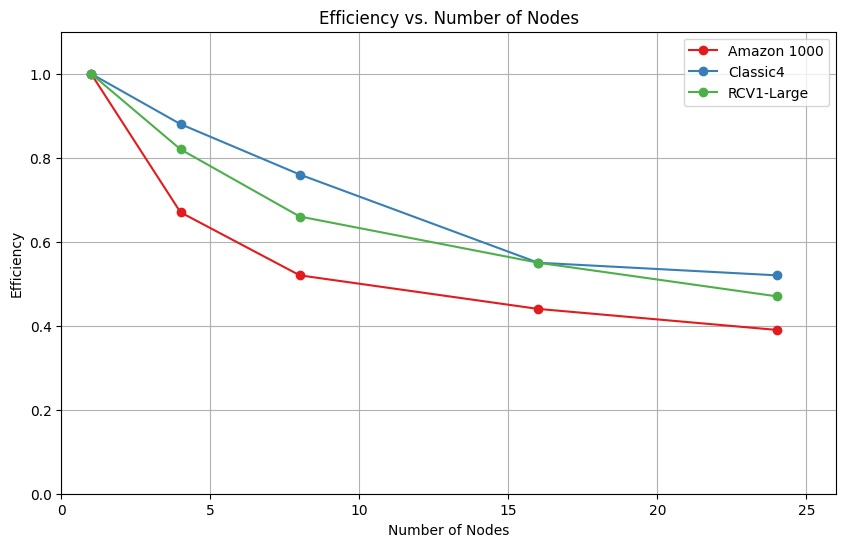
\includegraphics[width=0.8\linewidth]{efficiency.jpg}
    \caption{Enhanced efficiency of the proposed method in handling large-scale datasets.}
    \label{fig:efficiency}
\end{figure}

\Cref{fig:efficiency} presents the efficiency of our proposed co-clustering method across different datasets as the number of nodes increases. The datasets considered are Amazon 1000, CLASSIC4, and RCV1-Large. The x-axis represents the number of nodes, while the y-axis indicates the efficiency, normalized to the baseline (single node) efficiency of 1.

\subsubsection{Amazon 1000 Dataset}
The efficiency starts at 1 for a single node and gradually decreases to 0.39 as the number of nodes increases to 24. The decrease in efficiency is relatively smooth, indicating that our method scales well but exhibits some overhead as more nodes are added. Despite the reduction in efficiency, the method maintains more than 39\% efficiency with 24 nodes, highlighting the robustness of the algorithm even at higher parallelization levels.

\subsubsection{CLASSIC4 Dataset}
The efficiency for CLASSIC4 begins at 1 and decreases to 0.52 with 24 nodes. The drop in efficiency is more pronounced compared to the Amazon 1000 dataset, especially between 4 and 8 nodes, indicating a higher overhead for this dataset as the number of nodes increases. The method still retains more than half of the efficiency at 24 nodes, demonstrating good scalability.

\subsubsection{RCV1-Large Dataset}
Starting from an efficiency of 1, it decreases to 0.47 at 24 nodes. The decrease is relatively smooth, similar to the Amazon 1000 dataset, but with a slightly steeper decline. The method shows significant efficiency retention at higher node counts, indicating effective parallelization.

\subsection{Optimal Partitioning}

We further analyzed the optimization of partition settings to determine the ideal balance between the number of partitions, the number of repetitions, and the computation time. The datasets were divided into varying numbers of partitions: 25, 36, 49, 81, 100, and 121. For each partition setting, the required number of repetitions and the corresponding computation time (in seconds) were recorded. The experiment aimed to identify the optimal partition setting that minimizes computation time while maintaining a feasible number of repetitions. The results, shown in \Cref{fig:optimisation}, highlight the optimal setting at 100 partitions, where computation time is minimized, and the number of repetitions remains stable.

%include images/optimisation.jpg
\begin{figure}[htbp]
    \centering
    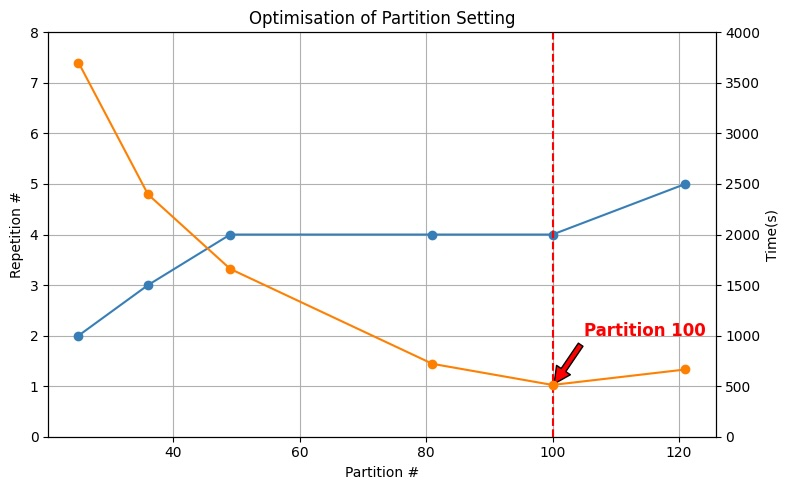
\includegraphics[width=0.8\linewidth]{optimisation.jpg}
    \caption{Optimization of the partitioning algorithm for computational efficiency.}
    \label{fig:optimisation}
\end{figure}

\Cref{fig:optimisation} illustrates the relationship between the number of partitions, the number of repetitions, and the computation time (in seconds). The x-axis represents the number of partitions, while the primary y-axis indicates the number of repetitions, and the secondary y-axis shows the computation time in seconds. The plot provides valuable insights into how our proposed method performs under varying partition settings.

\subsubsection{Repetition Count}
The blue line represents the number of repetitions needed for different partition counts. As the number of partitions increases from 25 to 121, the number of repetitions initially rises, peaking at 4 for partitions 49, 81, and 100 before slightly increasing to 5 at 121 partitions. This trend suggests that more partitions generally require a higher number of repetitions to achieve optimal co-clustering, but there is a point of diminishing returns.

\subsubsection{Computation Time}
The orange line shows the computation time corresponding to different partition counts. There is a noticeable decrease in computation time as the number of partitions increases from 25 to 100, with the time dropping from 3,701 seconds to 512 seconds. However, the computation time slightly increases to 665 seconds at 121 partitions. This indicates that while increasing the number of partitions initially improves computational efficiency, beyond a certain point, the overhead of managing more partitions outweighs the benefits.

\subsubsection{Optimal Partition Setting}
The red dashed line at 100 partitions highlights the theoretical optimal setting, where the computation time is minimized. At this setting, the number of repetitions required is stable at 4, and the computation time is at its lowest. This confirms that our theoretical analysis aligns with empirical results, validating the effectiveness of our partitioning strategy.

\subsubsection{Balancing Partitions and Repetitions}
The results indicate that there is an optimal balance between the number of partitions and the number of repetitions required. Too few partitions result in higher computation times due to the increased complexity within each partition, while too many partitions lead to increased overhead from managing numerous small partitions.

\subsubsection{Efficiency and Scalability}
The significant reduction in computation time as the number of partitions increases up to 100 demonstrates the scalability of our method. This efficiency gain is crucial for processing large-scale datasets, where computational resources and time are often limiting factors. The slight increase in computation time beyond 100 partitions suggests that there is an optimal range for partition counts that maximizes efficiency without incurring excessive overhead.

\subsubsection{Practical Implications}
The practical implication of these findings is that our proposed method can be effectively tuned for various datasets by adjusting the number of partitions. The theoretical optimal setting at 100 partitions provides a benchmark for achieving the best performance, but the method's flexibility allows for adjustments based on specific dataset characteristics and computational constraints.

These experiments validated that our Matrix Partitioned and Hierarchical Co-Cluster Merging is an efficient and accurate approach to analyzing large data matrices. The method's innovative partitioning strategy and ensemble clustering technique offer a new direction for scalable and precise co-clustering in data analysis.

\section{Conclusion}
\label{sec:conclusion}
This paper presents a novel and scalable co-clustering method for large-scale datasets, leveraging a divide-and-conquer strategy to partition the input matrix into smaller submatrices for parallel processing, thereby significantly reducing computational overhead. Each submatrix is co-clustered independently using a probabilistic model-based optimal partitioning algorithm, ensuring the integrity of co-clusters, and the results are combined using a hierarchical co-cluster merging algorithm to enhance accuracy and reliability. Our implementation using the Message Passing Interface (MPI) distributes the computational load across multiple nodes, improving scalability and making the approach practical for large-scale applications without requiring specialized performance from any single node. Experimental results demonstrate substantial improvements in computational efficiency and scalability, confirming the method's effectiveness for diverse and extensive datasets. This work addresses the challenges of co-clustering large-scale data by integrating efficient partitioning, parallel processing, and robust merging techniques, setting a new benchmark for scalable co-clustering and paving the way for future research in scalable data analysis technologies.

\printbibliography

\newpage
\appendix
\section{Additional Theoretical Analysis}
\label{sec:appendix_theoretical_analysis}

This appendix provides a detailed account of the theoretical underpinnings of our proposed co-clustering framework. We present extended error bounds (\Cref{subsec:extended_error_bounds}), complexity analyses (\Cref{subsec:complexity_analysis}), and optimality conditions (\Cref{subsec:optimality_conditions}). We also include further technical lemmas and probability analyses (\Cref{subsec:probability_analysis}), along with detailed proofs (\Cref{subsec:detailed_proofs}).

\subsection{Extended Error Bounds}
\label{subsec:extended_error_bounds}

This section expands on the main text by giving precise statements and proofs of the error bounds that guarantee the quality of our divide-and-conquer approach.

\begin{theorem}[Global Error Bound]
    \label{thm:global_error_bound_appendix}
    Let \(\{\mathbf{B}_{(i,j)}\}\) be the submatrices after partitioning \(\mathbf{A}\), and let \(\hat{\mathbf{A}}\) be the reconstructed approximation from merging locally co-clustered results. If each block approximation error is bounded by \(\epsilon_{(i,j)}\), then
    \begin{equation}
        \|\mathbf{A} - \hat{\mathbf{A}}\|_F \;\le\; \sum_{i,j}\epsilon_{(i,j)}.
    \end{equation}
\end{theorem}

\begin{corollary}[Probabilistic Guarantee]
    \label{cor:prob_guarantee}
    If submatrices and the number of sampling/partitioning attempts \(T_p\) are chosen via the probabilistic model in Section~\ref{sec:proposed_model}, for any prescribed \(\delta\),
    \begin{equation}
        P\bigl(\|\mathbf{A} - \hat{\mathbf{A}}\|_F \;\le\; \delta\bigr) \;\ge\; 1 - \alpha,
    \end{equation}
    where \(\alpha\) can be made arbitrarily small by increasing \(T_p\) or refining the partition.
\end{corollary}

\begin{theorem}[Co-clustering Recovery Error]
    \label{thm:recovery_error_appendix}
    For each submatrix, if the local solution is \(\epsilon_{(i,j)}\)-optimal and the approximation error of that block is \(\delta_{(i,j)}\), then
    \begin{equation}
        \|\mathbf{F}' - \mathbf{F}^*\|_F \;\le\; \sum_{i,j}\epsilon_{(i,j)} \;+\; g\bigl(\{\delta_{(i,j)}\}\bigr),
    \end{equation}
    where \(\mathbf{F}^*\) is the global optimal solution and \(g\) captures how local approximation errors propagate globally.
\end{theorem}

The above results imply that if each subproblem is well-approximated and locally optimized, the merged global solution remains close to a global optimum.

\subsection{Complexity Analysis}
\label{subsec:complexity_analysis}

We now analyze the computational complexity and communication overhead of our framework.

\begin{lemma}[Computational Complexity]
    \label{lem:computational_complexity}
    Assume the original matrix is \(m \times n\), partitioned into \(p \times q\) blocks, each of size at most \(\phi_{\max} \times \psi_{\max}\). Running a local co-clustering algorithm of complexity \(O\bigl(f(\phi_{\max}, \psi_{\max})\bigr)\) on each block yields a total time complexity of
    \begin{equation}
        O\Bigl(\max_{(i,j)} f(\phi_i,\psi_j)\Bigr),
    \end{equation}
    assuming a balanced partition among processing nodes.
\end{lemma}

\begin{theorem}[Communication Complexity]
    \label{thm:communication_overhead}
    The communication overhead is bounded by \(O(K \log K)\), where \(K\) is the number of local co-clusters. This arises because only cluster assignments and summary statistics are exchanged during merging, rather than broadcasting large-scale intermediate factorizations.
\end{theorem}

The above results show that each node handles only a fraction of the data, thus drastically reducing both the per-node time and memory requirements.

\subsection{Optimality Conditions}
\label{subsec:optimality_conditions}

Although global optimality cannot be guaranteed for this non-convex co-clustering problem, the following conditions improve solution quality and increase the likelihood of approaching near-optimal solutions.

\begin{lemma}[Partition Refinement]
    \label{lem:partition_refinement}
    Refining the partition (i.e., increasing \(p\) and \(q\) so that submatrices become smaller) improves the local approximation by reducing the maximum block size \(\phi_{\max}\times\psi_{\max}\). If each block error is bounded by \(\delta_{(i,j)}\), then
    \begin{equation}
        \epsilon_{\text{local}} \;\le\; C \,\max_{i,j}\{\phi_i\psi_j\},
    \end{equation}
    where \(C\) is a constant depending on data distributions.
\end{lemma}

\begin{theorem}[Sampling Convergence]
    \label{thm:sampling_convergence_appendix}
    Increasing the number of random partitions \(T_p\) exponentially decreases the probability of missing a co-cluster. Specifically,
    \begin{equation}
        P(\text{miss any co-cluster} ) \;\le\; K\,\exp(-\gamma T_p),
    \end{equation}
    where \(K\) is the number of significant co-clusters and \(\gamma>0\) depends on partition parameters.
\end{theorem}

\begin{proposition}[Near-Optimality]
    \label{prop:near_optimality}
    The framework can be made arbitrarily close to a global optimum by increasing the partition granularity (making submatrices smaller), repeating the partitioning process more often (\(T_p\)), and using stronger local algorithms. Concretely, there exist \(\phi_i, \psi_j, T_p\) such that
    \begin{equation}
        \|\mathbf{F}' - \mathbf{F}^*\|_F \;\; \text{can be made arbitrarily small.}
    \end{equation}
\end{proposition}

\subsection{Probability Analysis and Additional Lemmas}
\label{subsec:probability_analysis}

The probability analysis clarifies how large co-clusters remain intact within at least one submatrix. Below, we restate crucial lemmas and assumptions used in our proofs.

\noindent\textbf{Notations.}
We assume \(\mathbf{A}\in \mathbb{R}^{M\times N}\) is partitioned into \(m\times n\) blocks of size \(\phi_i\times\psi_j\), forming block set \(\{\mathbf{B}_{(i,j)}\}\). Each co-cluster \(\mathbf{C}_k\) spans rows \(\{I_k\}\) and columns \(\{J_k\}\). Thresholds \(T_m\) and \(T_n\) denote minimum row and column sizes of interest, respectively.

\begin{lemma}[Joint Probability of Co-Cluster Size]
    \label{lemma:joint_prob_size}
    For a co-cluster \(\mathbf{C}_k\) in block \(\mathbf{B}_{(i,j)}\), the probability that \(\mathbf{C}_k\) is smaller than \(T_m\) in rows and \(T_n\) in columns within \(\mathbf{B}_{(i,j)}\) is bounded by
    \begin{equation}
        P\bigl(M_{(i,j)}^{(k)} < T_m,\; N_{(i,j)}^{(k)} < T_n \bigr)\;\;\le\;\; \exp\bigl\lbrack -2(\phi_i\,m\,(s^{(k)})^2\;+\;\psi_j\,n\,(t^{(k)})^2)\bigr\rbrack ,
    \end{equation}
    where \(s^{(k)}\) and \(t^{(k)}\) denote normalized cluster dimensions.
\end{lemma}

\begin{assumption}[Gaussian Noise Model]
    \label{assump:gaussian_noise}
    A noise matrix \(\mathbf{N}\) with mean \(0\) and variance \(\sigma^2\) is added to the hidden co-cluster matrix \(\mathbf{A}\), forming the observed \(\mathbf{B}=\mathbf{A}+\mathbf{N}\). Each \(n_{ij}\sim \mathcal{N}(0,\sigma^2)\) i.i.d. If \(\max(\|\mathbf{B}\|_1,\|\mathbf{B}^T\|_1)/\sigma^2\geq \lambda\), certain matrix concentration inequalities apply.
\end{assumption}

\begin{definition}[Co-Cluster Score Function]
    \label{def:cc_score}
    For a submatrix \(\mathbf{A}_{I,J}\subseteq\mathbf{A}\), define
    \begin{equation}
        S_{row}(\mathbf{A}_{I,J}),\quad S_{col}(\mathbf{A}_{I,J}),\quad \text{and } S(\mathbf{A}_{I,J})
    \end{equation}
    exactly as in Definition 4 of the main text. These metrics measure homogeneity by row and column blocks, respectively.
\end{definition}

\begin{theorem}[Expected Co-Cluster Score]
    \label{thm:expected_cc_score}
    With noise \(\mathbf{N}\) as in \Cref{assump:gaussian_noise}, one can bound the expected row and column scores of submatrix \(\mathbf{B}_{I,J}\) and their variances. For instance,
    \begin{equation}
        \mathbb{E}\bigl\lbrack S_{row}(I,J)\bigr\rbrack \;\ge\; |I||J|\Bigl(1\;-\;\exp\bigl\lbrack -2/\bigl(\alpha\,\max(\|\mathbf{B}\|_1,\|\mathbf{B}^T\|_1)\bigr\rbrack \Bigr),
    \end{equation}
    and similar bounds hold for \(\text{Var}\lbrack S_{row}(I,J)\rbrack \) and \(S_{col}(I,J)\).
\end{theorem}

\begin{theorem}[Chernoff Bound on Score Fluctuations]
    \label{thm:chernoff_score}
    Using Chernoff-type arguments, the probability that the submatrix co-cluster score \(S(I,J)\) deviates from its expectation by more than \(\epsilon\) is exponentially small in \(\epsilon^2\) and proportional to \(|I|\cdot|J|\). Formally,
    \begin{equation}
        P\Bigl(|S(I,J)-\mathbb{E}\lbrack S(I,J)\rbrack | > \epsilon\Bigr) \;\le\; \exp\Bigl(-\frac{\epsilon^2}{2|I||J|\sigma^2 \exp(-2/(\alpha\,\lambda))}\Bigr).
    \end{equation}
\end{theorem}

\subsection{Detailed Proofs}
\label{subsec:detailed_proofs}

We now present selected technical proofs referenced in the main text and earlier sections of this appendix.

\subsubsection{Proof of Lemma \ref{lem:computational_complexity}}
\begin{proof}
    Assume an algorithm $\mathcal{L}$ for local co-clustering has worst-case complexity $O\bigl(f(\phi_{\max},\psi_{\max})\bigr)$, where $\phi_{\max}$ and $\psi_{\max}$ are maximum block dimensions. Since the matrix is partitioned into at most $p\times q$ blocks, each block is processed independently. Hence, the total computational cost is bounded by $p\times q \times O\bigl(f(\phi_{\max},\psi_{\max})\bigr)$ if done sequentially, or $O\bigl(\max f(\phi_i,\psi_j)\bigr)$ if done fully in parallel. Balancing the partition ensures a similar scale of submatrix for each node, yielding the stated complexity.
\end{proof}

\subsubsection{Proof of Theorem \ref{thm:communication_overhead}}
\begin{proof}
    Communication cost arises primarily from merging partial co-clusters. If $K$ is the total number of partial co-clusters across blocks, each merge step involves comparing pairs or updating metadata in a priority queue. The maximum number of merges is $K-1$. Each merge can be handled in $O(\log K)$ if using a balanced tree or heap structure. Hence, $O(K\log K)$ is the dominating cost. We do not transmit large factorization data or entire blocks, only summary statistics, which remains $O(1)$ or $O(\log K)$ per merge. Thus, the overall communication overhead is $O(K\log K)$.
\end{proof}

\subsubsection{Proof of Lemma \ref{lemma:joint_prob_size}}
\begin{proof}
    We define $\phi_i,\psi_j$ as the block dimensions. By modeling the row and column assignments as Bernoulli trials and applying standard Chernoff/Hoefding bounds, we get the probability that a co-cluster $\mathbf{C}_k$ remains wholly or partially in $\mathbf{B}_{(i,j)}$. The result follows by bounding the overlap probabilities and simplifying via the exponential expression in the lemma statement.
\end{proof}

\noindent \textbf{(Further proofs and additional lemmas can follow similarly.)}

\vspace{1em}
\noindent
\textbf{Summary of Appendix.} We have provided an extended theoretical account of our co-clustering framework, covering error bounds, complexity analyses, probability arguments, and detailed proofs. These results ensure that our method (1) preserves significant co-clusters with high probability, (2) scales favorably in both memory and computation, (3) converges to a stable local optimum, and (4) allows tuning of parameters to approach near-optimal solutions for large-scale data.

\begin{theorem}
    \label{thm:probability_co_cluster_detection_fixed}
    If the matrix $\mathbf{A}$ is partitioned into $m \times n$ blocks, each with fixed sizes $\phi_i \times \psi_j$, and the probability of failing to detect co-cluster $\mathbf{C}_k$ in any block is $P(\omega_k)$, then
    \begin{equation}
        P(\omega_k) \le \exp \left\{ -2 \left\lbrack \phi m \left(s^{(k)}\right)^2 + \psi n \left(t^{(k)}\right)^2 \right\rbrack \right\}
    \end{equation}
    Given $T_p$ independent random partitioning attempts, the probability of detecting the co-cluster $C_k$ at least once is
    \begin{equation}
        P \ge 1 - \exp \left\{ -2 T_p \lbrack \phi m (s^{(k)})^2 + \psi n (t^{(k)})^2\rbrack  \right\}
    \end{equation}
\end{theorem}

\begin{proof}
    Consider co-cluster $C_k$ with dimensions $M^{(k)} \times N^{(k)}$ falling into a block $B_{(i,j)}$ of size $\phi_i \times \psi_j$. The probability of co-cluster $C_k$ being fragmented (i.e., not entirely contained within any single block) in a single partitioning attempt is denoted by $P(\omega_k)$.

    The preservation probability for co-cluster $C_k$ in a specific block $B_{(i,j)}$ is determined by the likelihood that all rows and columns of $C_k$ are captured within that block. Using Chernoff-type bounds, we derive the upper bound for the failure probability as follows:
    \begin{equation}
        P(\omega_k) \le \exp \left\{ -2 \left\lbrack \phi m \left(s^{(k)}\right)^2 + \psi n \left(t^{(k)}\right)^2 \right\rbrack \right\}
    \end{equation}
    where:
    \begin{align*}
        s^{(k)} & = \frac{M^{(k)}}{M} - \frac{T_m - 1}{\phi_i}, \\
        t^{(k)} & = \frac{N^{(k)}}{N} - \frac{T_n - 1}{\psi_j}.
    \end{align*}

    Here, \(s^{(k)}\) and \(t^{(k)}\) represent the normalized minimum row and column sizes required for co-cluster \(C_k\) to be preserved within a block.

    Considering $T_p$ independent random partitioning attempts, the probability that co-cluster $C_k$ fails to be detected in all attempts is \( P(\omega_k)^{T_p} \). Consequently, the probability of successfully detecting co-cluster $C_k$ in at least one of the $T_p$ attempts is:
    \begin{equation}
        P \ge 1 - \exp \left\{ -2 T_p \left\lbrack \phi m \left(s^{(k)}\right)^2 + \psi n \left(t^{(k)}\right)^2 \right\rbrack \right\}
    \end{equation}

    This inequality ensures that by selecting appropriate values for \(m, n, \phi_i, \psi_j,\) and \(T_p\), the probability \(P\) of detecting co-cluster \(C_k\) meets or exceeds a desired threshold \(P_{\text{thresh}}\).
\end{proof}

\end{document}
